\chapter{Comportamientos emergentes }\label{cap:modeloneuronal}
\graphicspath{{figs/capitulo_introduccion_robot/}}

\chapterquote{Far from being able to accept the idea of the individuality and independence of  	each nerve element, I have never had reason, up to now, to give up the concept 	which I have always stressed, that nerve cells, instead of working individually, act 	together [...]. However opposed it may seem to the popular tendency to individualize the elements, I cannot abandon the idea of a unitary action of the 	nervous system [...]}{Camillo Golgi, 1906}




En un entorno complejo, dinámico y altamente competitivo, la supervivencia de los sistemas biológicos exige la toma de una amplia gama de decisiones relativas a sus actividades potenciales. Esta necesidad de optimización en la toma de decisiones, bajo la constante presión evolutiva, ha propiciado la inevitable explotación de procesos de procesamiento de información, a menudo referidos como \textquote{computación} \cite{baluska_having_2016}. 


El comportamiento de un organismo se origina en la  actividad coordinada de un conjunto diverso de neuronas interconectadas.  La cantidad de estas neuronas varía significativamente entre especies, desde unas 302 en Caenorhabditis elegans hasta varios miles de millones en seres humanos. La determinación de la conectividad entre estas neuronas, conocida como el \textquote{Conectoma}, ha sido una piedra angular en la neurociencia y se ha basado en la combinación de enfoques anatómicos y electrofisiológicos. Esto ha implicado la visualización detallada de las estructuras especializadas de la membrana y las vesículas sinápticas en las sinapsis a través de la microscopía electrónica de secciones cerebrales seriadas.

Además, se ha avanzado en el análisis de la actividad electrofisiológica con el fin de comprender la operación de las sinapsis y circuitos neuronales con una resolución más alta. Este enfoque se ha ampliado progresivamente para incluir un mayor número de neuronas interconectadas. En este contexto, se han desarrollado diversas perspectivas y teorías para arrojar luz sobre la intrincada relación entre la estructura y la función en las redes neuronales.

Uno de los hallazgos más notables es la observación de que las redes neuronales, al igual que muchas otras redes biológicas, presentan importantes propiedades estructurales. En particular, el análisis de características como el coeficiente de agrupamiento y la longitud de camino característica ha revelado que estas redes siguen una topología de mundo pequeño, caracterizada por distancias relativamente cortas entre cualquier par de nodos \cite{heuvel_comparative_2016}. Además, se ha observado que estas redes siguen una distribución de grados que obedece a una ley de potencia, en la que la mayoría de las neuronas se conecta con un número limitado de nodos, mientras que una pequeña fracción de neuronas establece conexiones con un número excepcionalmente alto de otras neuronas \cite{varshney_structural_2011}.

Un enfoque alternativo se centra en la identificación de bloques de construcción recurrentes incrustados en la estructura de estas redes, denominados \textquote{motivos de red}. Se ha demostrado que estos motivos de red están significativamente sobrerrepresentados en las redes biológicas, incluyendo la red neuronal de Caenorhabditis elegans (C. elegans) \cite{milo_network_2002}. Al explorar estos motivos, se ha logrado discernir sus posibles funciones en la red y cómo contribuyen a la generación de comportamientos emergentes. En los últimos años, se ha profundizado en un fenómeno intrigante conocido como la \textquote{regla del vecino común} (CNR), que sugiere que la probabilidad de conexión entre dos neuronas es mayor cuando comparten un mayor número de vecinos comunes. Esta organización da lugar a la formación de subredes relativamente independientes, incrustadas en la arquitectura de la red a gran escala. Investigaciones recientes, como las de Azulay et al. \cite{azulay_c_2016}, han demostrado que la CNR es una propiedad emergente en la red neuronal de C. elegans, y que los conjuntos de vecinos comunes forman estructuras homogéneas en capas definidas de la red, lo que confiere importantes roles funcionales.



A pesar de su aparente simplicidad, C. elegans exhibe una amplia gama de comportamientos complejos. Por ejemplo, explora su entorno mediante movimientos sinusoidales entrecortados por giros rápidos o bruscos, denominados \textquote{piruetas}. Al tocar al gusano, desencadena de manera predecible una respuesta de inversión \cite{bono_neuronal_2005}. Además, otros estímulos, como sustancias químicas que sugieren la presencia de alimento, pueden inducir cambios más estocásticos, como el aumento de la probabilidad de realizar piruetas cuando se percibe una disminución en la cantidad de comida cercana.


Estos patrones de comportamiento permiten a los gusanos explorar su entorno y adaptarse a las condiciones cambiantes, dificultando su muerte por parte de depredadores. Así, surge la pregunta: ¿cómo genera C. elegans secuencias de comportamiento variables? ¿Cómo integra la diversa información sensorial para ajustar las probabilidades de sus comportamientos? Estas cuestiones representan un desafío central en la neurociencia de sistemas, tanto en el contexto de los gusanos como en la ciencia en general \cite{branson_imaging_2015}.

Para responder a estas interrogantes, en los últimos años  se utilizó el conectoma de C. elegans para identificar las neuronas necesarias para la respuesta de evitación del tacto, que es el comportamiento más completamente caracterizado del animal. El análisis se basó en la eliminación selectiva de células mediante un microhaz láser y la evaluación del repertorio conductual resultante. Siguiendo el diagrama de conexiones neuronales, se logró identificar las neuronas mecano-sensoriales esenciales ubicadas en la cabeza y la cola, las interneuronas clave necesarias para propagar la información, y las neuronas motoras necesarias para el movimiento hacia adelante y hacia atrás. Este enfoque exitoso motivó análisis similares de otros comportamientos, como los relacionados con la detección de sustancias químicas, la alimentación y la puesta de huevos. Actualmente, se ha definido la función de más del 60 \% de los tipos de neuronas en C. elegans en uno o varios comportamientos \cite{bargmann_connectome_2013}.


No obstante, este éxito oculta un sorprendente fracaso. A pesar de que sabemos qué hacen la mayoría de las neuronas, no comprendemos las funciones de la mayoría de las conexiones ni podemos predecir fácilmente la importancia funcional de estas conexiones basándonos únicamente en el diagrama de conexiones. Esta discrepancia general entre el número de sinapsis y su aparente importancia funcional se manifiesta en todos los circuitos de C. elegans. Como resultado, las primeras suposiciones sobre cómo podría fluir la información a través del diagrama de conexiones resultaron en gran medida incorrectas \cite{bargmann_connectome_2013}.


Es evidente que el diagrama de conexiones, por sí solo, no puede proporcionar información adecuada para predecir la salida fisiológica de los circuitos. Los canales, las sinapsis y los procesos bioquímicos interactúan para generar características explícitamente definidas en el tiempo, o dinámicas, en las neuronas y los circuitos. El análisis de la dinámica neuronal a menudo requiere la monitorización y la manipulación simultánea de los circuitos. Las técnicas emergentes de optogenética y farmacogenética se han desarrollado para abordar este problema \cite{kato_global_2015}.


Para complementar y respaldar estos enfoques experimentales, es esencial desarrollar modelos que describan cómo el resultado de un sistema surge de las interacciones entre sus componentes. Existe una tensión entre el deseo de estudiar modelos abstractos adecuados para análisis matemáticos precisos y el deseo de estudiar modelos lo suficientemente realistas desde una perspectiva biológica como para representar las estructuras y funciones subyacentes del sistema. 

Dado lo anterior, es importante considerar el sistema nervioso en su totalidad al estudiar el comportamiento. Esto se debe a que los circuitos interactúan entre sí para generar comportamiento, y el estudio de partes aisladas del sistema nervioso puede resultar insuficiente para comprender su funcionamiento global. Además, muchas de las dinámicas clave que permiten el procesamiento de información pueden ser implementadas por diferentes componentes biológicos. Es posible que los motivos de red mencionados previamente realicen una computación canónica o unas pocas computaciones canónicas, de modo que la resolución de algunos de estos motivos podría resolver eficazmente una parte sustancial del diagrama.

En el contexto de las investigaciones previamente mencionadas, se ha explorado a fondo la compleja red neuronal de Caenorhabditis elegans (C. elegans). Sin embargo, a pesar de los avances significativos en la identificación de las funciones de las neuronas individuales y las características de las conexiones sinápticas, persisten incógnitas cruciales sobre cómo estas conexiones se traducen en comportamientos observables en el organismo. Esta discrepancia fundamental entre la estructura neuronal y la función conductual plantea un desafío intrigante en el campo de la neurociencia.

Para abordar este desafío y avanzar en nuestra comprensión de cómo emerge el comportamiento a partir de la compleja red neuronal de C. elegans, se propone la utilización de un enfoque novedoso: la implementación de un modelo robótico . Este modelo, definido como una entidad mecánica y electrónica, capaz de interactuar con su entorno y llevar a cabo secuencias de comportamientos  \cite{brambilla_swarm_2013}, nos permitirá investigar cómo las características estructurales y funcionales de la red neuronal se traducen en respuestas conductuales.

En el corazón de este enfoque se encuentra la idea de que la red neuronal de C. elegans, con su conectoma, puede ser emulada en un robot. El robot, equipado con una representación precisa del conectoma y una dinámica neuronal adecuada, servirá como un modelo experimental en el que podremos observar y manipular las interacciones entre neuronas y circuitos con un alto grado de control. Esta aproximación nos permite explorar cómo las propiedades estructurales de la red neuronal influyen en la generación de comportamientos específicos y cómo la información sensorial es procesada y utilizada para modular respuestas conductuales.

La elección de utilizar un modelo robótico presenta varias ventajas distintivas. En primer lugar, nos brinda la capacidad de acceder y controlar completamente los aspectos computacionales y algorítmicos que gobiernan el comportamiento del modelo, lo que no es posible en el organismo vivo. Esto permite realizar experimentos sistemáticos y reproducibles, lo que es esencial para investigaciones rigurosas.

En segundo lugar, el modelo robótico nos otorga la capacidad de llevar a cabo experimentos en un entorno controlado y predecible, lo que simplifica la observación y el análisis de los resultados. Esta característica es esencial para comprender las relaciones causales entre la estructura de la red neuronal y el comportamiento. 

Por último, el uso de robots nos ofrece la flexibilidad de modificar y explorar diferentes aspectos del modelo, lo que nos permitirá realizar experimentos variados y diseñados específicamente para abordar preguntas de investigación concretas. Además, el modelo robótico es completamente independiente de los desafíos éticos y técnicos asociados con la manipulación de un organismo vivo.

Este capítulo tiene como objetivo ahondar en las bases neurobiológicas de Caenorhabditis elegans (C. elegans), centrándonos en su sistema nervioso, experimentos optogenéticos y modelos encontrados en la literatura. El propósito principal es proporcionar un sólido marco de referencia que facilite la comprensión de las investigaciones y resultados presentados en los capítulos posteriores. Exploraremos las estructuras neuronales clave y analizaremos los experimentos que han arrojado luz sobre la relación entre la estructura del sistema nervioso de C. elegans y su comportamiento. Además, revisaremos los modelos y teorías previas que respaldan nuestras investigaciones, contribuyendo así a una comprensión más profunda del organismo.   Al final del capítulo, se plantean los interrogantes que se desean resolver mediante nuestro modelo robótico y las hipótesis planteadas para dar solución a estas preguntas. Es importante destacar  que la implementación de un modelo robótico basado en el conectoma de C. elegans y una dinámica neuronal adecuada representa un enfoque prometedor para investigar las complejas interacciones entre la estructura de la red neuronal y la generación de comportamientos. A través de este modelo, buscamos arrojar luz sobre los mecanismos subyacentes que conectan la topología de la red con la función neural y, finalmente, con la conducta observada. Este enfoque no solo mejorará nuestra comprensión de la neurobiología de C. elegans, sino que también tiene el potencial de aportar conocimientos valiosos para el diseño y el control de sistemas robóticos basados en principios biológicos.



\section{Aspectos biológicos del C. elegans}

En este apartado, se expondrán los aspectos biológicos más significativos del organismo modelo conocido como Caenorhabditis elegans (C. elegans).  Su tamaño es modesto, con un cuerpo transparente que mide aproximadamente \qty{1}{\milli\metre } y un ciclo de vida que se completa en tan solo 3 días. A lo largo de su desarrollo, pasa por cuatro estadios larvarios (L1-L4) antes de alcanzar la edad adulta, la cual se caracteriza por una longevidad de 2-3 semanas a una temperatura de  \qty{20}{\degreeCelsius} \cite{yue_caenorhabditis_2021}. En el laboratorio, se puede mantener fácilmente en medios sólidos o líquidos utilizando E. coli OP50, una bacteria no patógena, como fuente de alimento.

Cabe destacar que C. elegans presenta dos sexos naturales bien definidos: el hermafrodita (XX) y el macho (XO). Los hermafroditas son capaces de reproducirse por autofecundación, generando aproximadamente 300 crías en cada ciclo reproductivo, con una proporción muy baja de machos (0.1\%). Esta característica facilita la producción de progenie genéticamente idéntica. Además, se ha secuenciado su genoma, y más del 65\% de sus genes tienen homólogos relacionados con enfermedades humanas. La \Cref{fig:sistema_anatomia}  resume las características anatómicas clave de C. elegans, que se caracteriza por una anatomía simple con un número limitado de tejidos y órganos. La mayoría de los estudios de comportamiento se han centrado en hermafroditas, a excepción de aquellos que investigan el apareamiento.

Tanto en hermafroditas como en machos, el número de células corporales es preciso, con 959 núcleos somáticos en hermafroditas y 1031 en machos. Estas células contribuyen a la formación de la hipodermis, el músculo, el tracto digestivo, la gónada y el sistema nervioso.

 \begin{figure}[h!]
	\centering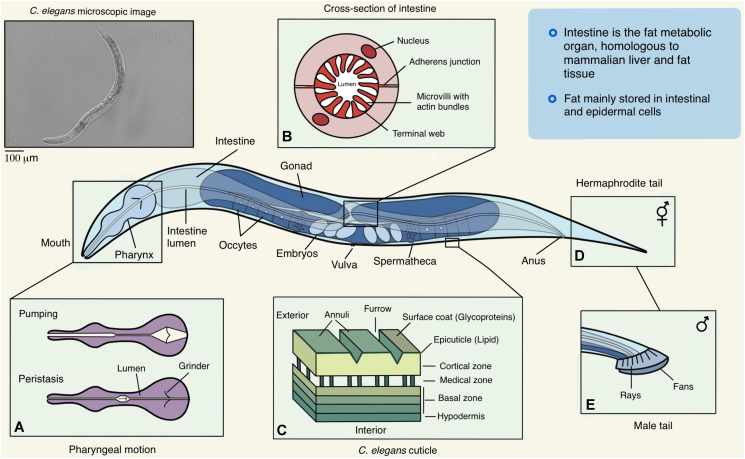
\includegraphics[width=\imsize]{gr1.jpg}
	\caption[ Anatomía del Caenorhabditis elegans adulto.]{ Anatomía del Caenorhabditis elegans adulto.La figura ilustra la anatomía fundamental del organismo modelo, Caenorhabditis elegans (C. elegans), que es crucial para contextualizar sus características biológicas. La anatomía básica de C. elegans comprende varios componentes esenciales. (A) La boca está formada por seis labios simétricos que crean una cavidad circular de \qtyrange{1}{2}{\micro\metre}, facilitando la ingestión de alimento que se dirige al órgano de alimentación, la faringe. (B) El intestino se compone de 20 células epiteliales grandes organizadas bilateralmente en pares simétricos para formar un tubo largo con un lumen central. (C) La cutícula, que en adultos jóvenes tiene un grosor de aproximadamente \qty{0.5}{\micro\metre}, consta de cuatro capas principales: epicutícula, cortical, medial y basal. (D y E) La cola de la hermafrodita se estrecha hacia un extremo afilado, mientras que la cola del macho se caracteriza por ser roma y contiene un aparato copulador distintivo.  (Adaptado de \protect\cite{yue_caenorhabditis_2021} ).}\label{fig:sistema_anatomia}
\end{figure}



\subsection{Sistema nervioso}





En el campo de la neurobiología, la comprensión de cómo el sistema nervioso desempeña sus funciones integrativas e instructivas es de suma importancia. El sistema nervioso es una red compleja de neuronas interconectadas, y la transmisión de actividad entre estas neuronas es esencial para su funcionamiento. Las sinapsis químicas y eléctricas son los elementos clave a través de los cuales la actividad de una neurona se comunica con otras. Además, cada neurona normalmente recibe entradas de múltiples neuronas presinápticas, y las interacciones entre estas entradas son cruciales para determinar la respuesta de la neurona postsináptica. Por consiguiente, la estructura de la red y las propiedades de las sinapsis son los principales determinantes del flujo de información en el sistema nervioso \cite{toyoshima_deducing_2022}.

En el caso específico de C. elegans, encontramos dos sistemas nerviosos prácticamente independientes. El sistema nervioso somático, presente en el hermafrodita adulto, consta de 302 neuronas agrupadas en 118 clases distintas, mientras que el sistema nervioso faríngeo, que se encarga de la alimentación, comprende 20 neuronas distribuidas en 14 clases. Estos dos sistemas nerviosos están conectados por una única conexión sináptica eléctrica entre las neuronas RIP somáticas y las neuronas I1 faríngeas \cite{fang-yen_illuminating_2015}. Por otro lado, los machos de C. elegans poseen 381 neuronas y 92 células gliales y de soporte. Aproximadamente la mitad de las neuronas se ubican en la cabeza, rodeando un neuropilo central denominado anillo nervioso, mientras que el resto se distribuye a lo largo del cordón ventral y en los ganglios de la cola. Las neuronas específicas de los machos se encuentran principalmente en la cola copulatoria. En ambos sexos, cada neurona se identifica de manera única en diferentes individuos por su posición y morfología característica.

Las neuronas de C. elegans se designan mediante un código de 2 o 3 letras, acompañado en ocasiones de un número, seguido generalmente de letras L (izquierda), R (derecha), D (dorsal) o V (ventral) para especificar su posición anatómica. Estas neuronas se pueden clasificar como sensoriales, interneuronas y motoras, en función de sus características anatómicas y su conectividad sináptica (\Cref{fig:conectoma_a, fig:sistema_nervioso2}). Las neuronas sensoriales poseen terminaciones sensoriales, ya sea que se haya demostrado su funcionalidad o no. Las neuronas motoras establecen sinapsis con células musculares, mientras que las interneuronas forman numerosas conexiones con otras neuronas. No obstante, estas categorías son en cierta medida arbitrarias, ya que muchas neuronas abarcan dos o más funciones. Por ejemplo, las neuronas motoras excitadoras de tipo B establecen sinapsis con diversas neuronas y, además, se ha demostrado que desempeñan una función sensorial propioceptiva. Para obtener una lista completa de las neuronas de C. elegans, su linaje y descripciones detalladas, se puede consultar la base de datos WormAtlas (\url{https://www.wormatlas.org/}).


 \begin{figure}[h!]
	\centering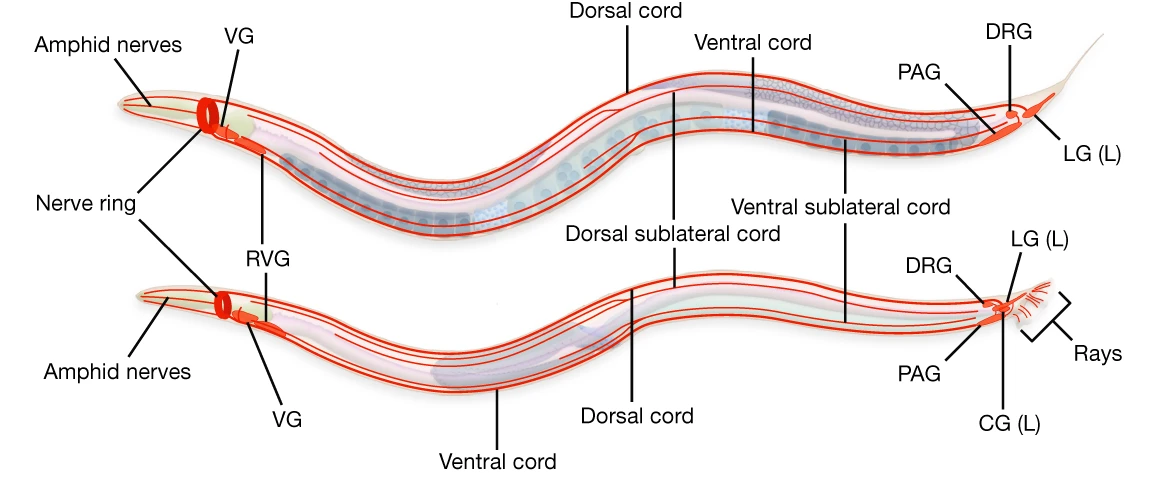
\includegraphics[width=\imsizeL]{conectoma_a.png}
	\caption[Representación del Sistema Nervioso de Caenorhabditis elegans.]{ Representación del Sistema Nervioso de Caenorhabditis elegans. En el hermafrodita adulto y el macho adulto, se destacan los principales ganglios y tractos nerviosos, dispuestos desde el extremo anterior hacia el izquierdo. De particular relevancia son los centros neurales de conectividad, entre los que se incluyen el anillo nervioso y, exclusivamente en el macho, el ganglio preanal. Se han identificado y etiquetado áreas significativas, tales como el ganglio cloacal (CG), el ganglio dorsorrectal (DRG), el ganglio lumbar (LG), el ganglio preanal (PAG), el ganglio retrovesicular (RVG) y el ganglio ventral (VG).   (Figura adaptada de \protect\cite{cook_whole-animal_2019}).}\label{fig:conectoma_a}
\end{figure}


 \begin{figure}[h!]
	\centering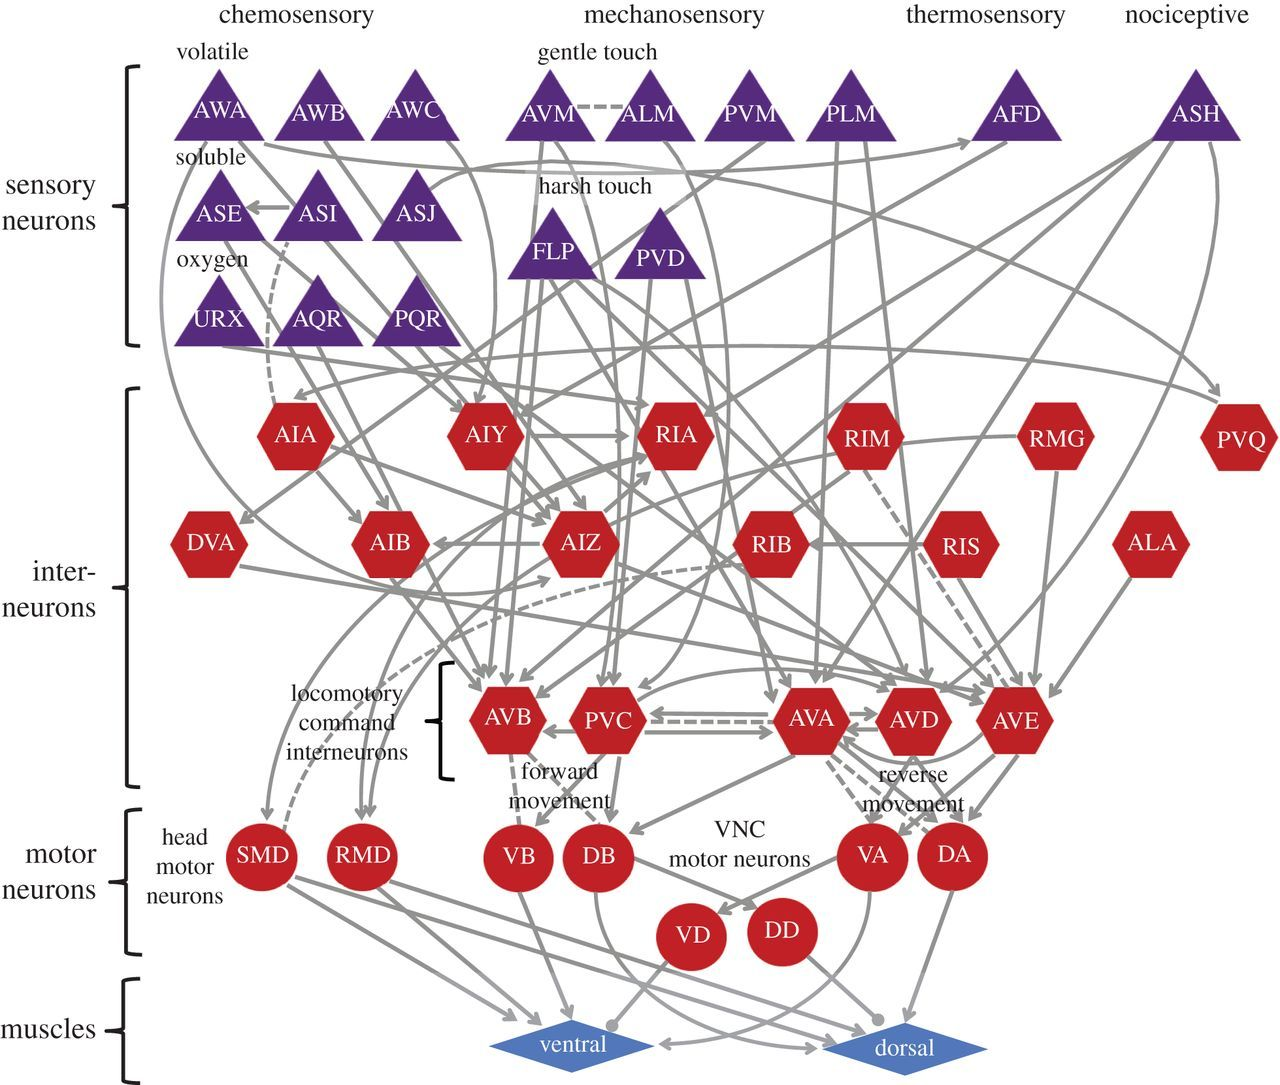
\includegraphics[width=\imsize]{rstb20140212f02.jpg}
	\caption[ Diagrama del circuito parcial del sistema nervioso somático y la musculatura de C. elegans. ]{ Diagrama del circuito parcial del sistema nervioso somático y la musculatura de C. elegans.  En el diagrama, se representan las neuronas sensoriales mediante triángulos, las interneuronas mediante hexágonos, las neuronas motoras mediante círculos y los músculos mediante diamantes. Las flechas indican conexiones sinápticas, que pueden ser de naturaleza excitatoria o inhibitoria, mientras que las líneas discontinuas señalan conexiones mediante sinapsis eléctricas. El cordón nervioso ventral (VNC) se identifica como una parte fundamental del sistema.  (Adaptado de \protect\cite{shibue_deconvolution_2020}).}\label{fig:sistema_nervioso2}
\end{figure}


\subsection{Locomoción}

La investigación en el comportamiento de Caenorhabditis elegans (C. elegans) se ha enfocado principalmente en el procesamiento sensorial de los estímulos ambientales que influyen en el patrón de locomoción de estos nematodos. La locomoción en C. elegans se lleva a cabo mediante un mecanismo de propulsión ondulatoria, caracterizado por la generación de un tren de ondas que se propaga a lo largo del cuerpo del gusano. La orientación del gusano, ya sea en su lado izquierdo o derecho, determina la formación de estas ondas, que resultan de la secuencia de contracciones y relajaciones alternas de los músculos longitudinales en la pared corporal, tanto dorsal como ventral. Tres fuerzas fundamentales permiten el movimiento en superficies sólidas: el esqueleto hidrostático, que sirve como punto de apoyo para la acción muscular; la tensión superficial, que presiona al gusano contra su sustrato; y la fricción entre el gusano y su superficie de apoyo, que permite que las ondas corporales avancen sin deslizamiento, generando así la propulsión hacia adelante.

El sistema muscular responsable de la locomoción en C. elegans comprende 95 células musculares de la pared corporal que reciben entradas excitatorias a través de uniones neuromusculares colinérgicas (NMJ) y entradas inhibitorias a través de NMJ GABAérgicas \cite{bono_neuronal_2005}. Diferentes clases de neuronas motoras distribuidas a lo largo del cuerpo regulan diferentes regiones de la musculatura. Un conjunto de neuronas dorsales (DB, DD) y ventrales (VB, VD), tanto excitatorias como inhibitorias, controla el movimiento hacia adelante, mientras que otro conjunto de neuronas (DA, DD y VA, VD) gobierna el movimiento hacia atrás. La interconexión de estas neuronas implica que, por ejemplo, la excitación de las neuronas motoras colinérgicas ventrales, como VB o VA, en una región específica de la musculatura ventral, resulta en la relajación de la musculatura dorsal opuesta debido a la inhibición de las neuronas motoras GABAérgicas (DD). Esto lleva a una curvatura específica del cuerpo. Esta inhibición recíproca es de suma importancia, especialmente en los movimientos de escape rápidos (\Cref{fig:movimiento}).



 \begin{figure}[h!]
	\centering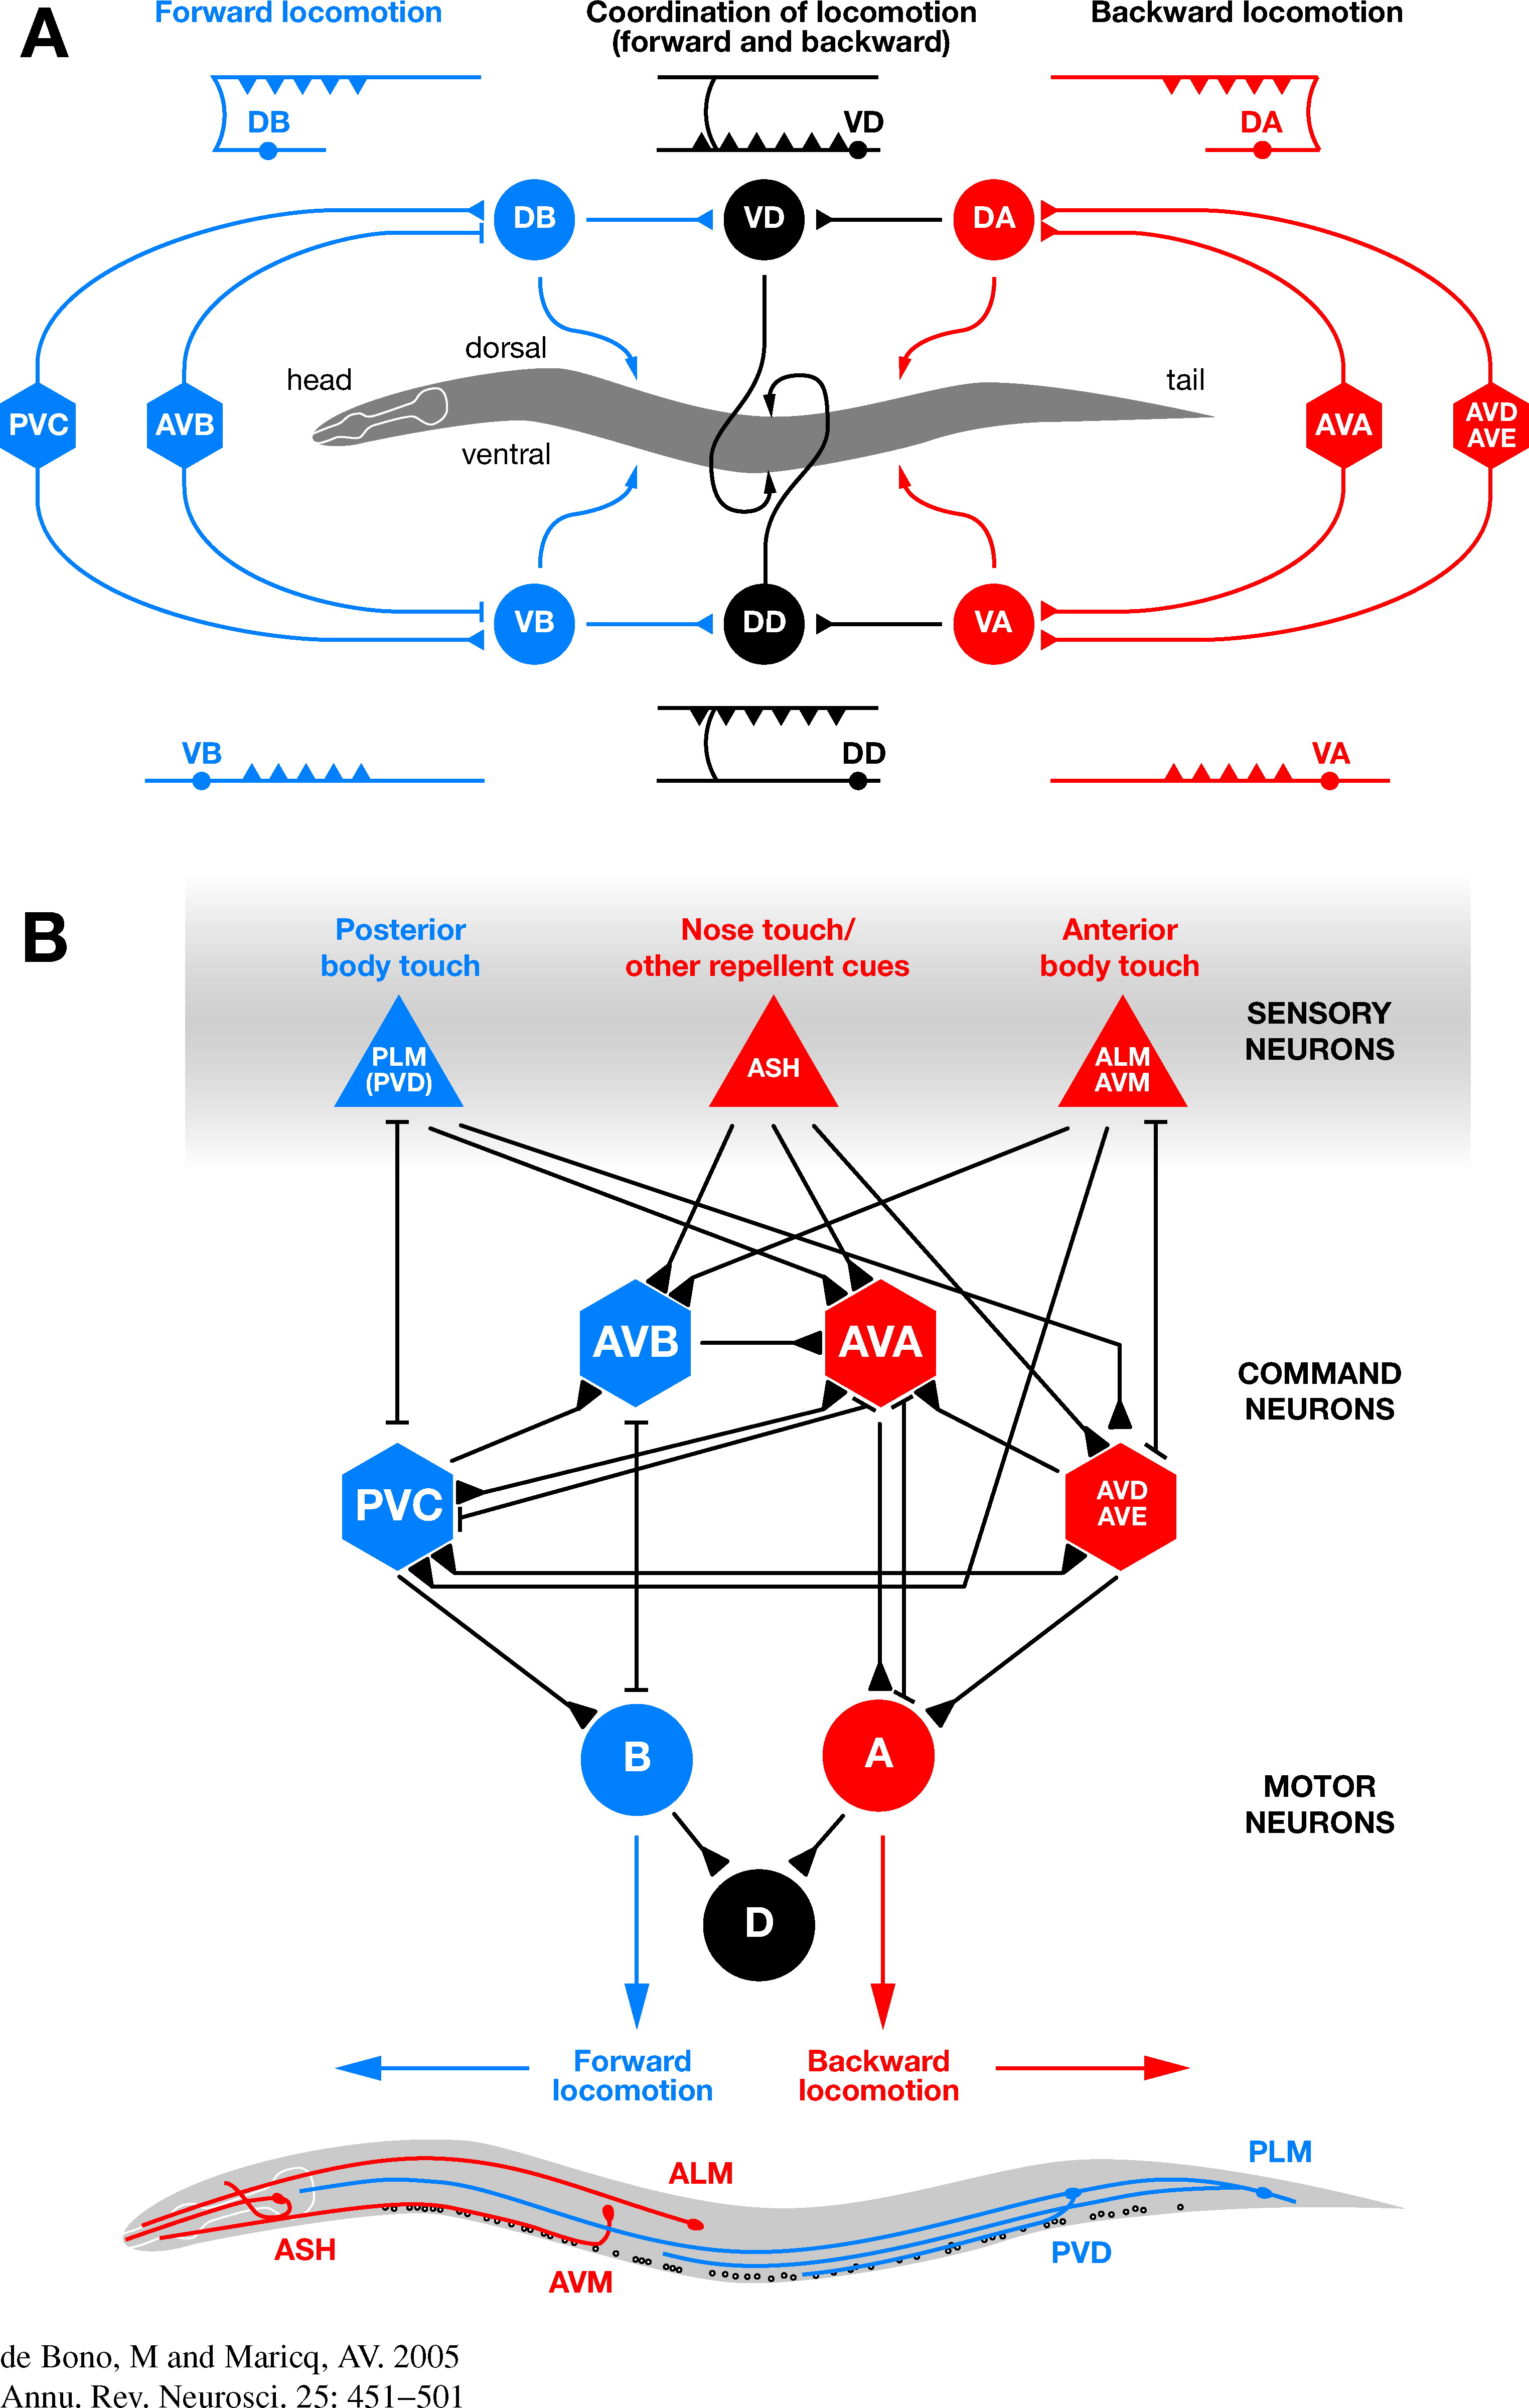
\includegraphics[width=\imsize]{ne280451.f1.jpeg}
	\caption[ Control Neuronal de la Locomoción hacia Adelante y Hacia Atrás ]{ Control Neuronal de la Locomoción hacia Adelante y Hacia Atrás. A) En este diagrama, se detalla la compleja conectividad entre las interneuronas de comando (hexágonos) y las neuronas motoras (círculos). Las sinapsis químicas se indican mediante triángulos, mientras que las eléctricas se representan mediante barras. Los pequeños círculos reflejan los cuerpos celulares, y las líneas representan los procesos neuronales, destacando las sinapsis de las neuronas motoras. Todos los cuerpos celulares se ubican en el lado ventral del gusano. 	B) El circuito que regula la respuesta al tacto, fundamental en la generación de movimientos de avance y retroceso, se ilustra en el diagrama superior. Se resalta la conectividad entre las neuronas sensoriales (triángulos), las interneuronas de comando y las neuronas motoras. Las neuronas PVD desempeñan un papel esencial en la respuesta a estímulos táctiles intensos, mientras que las neuronas PLM, ALM y AVM son críticas para las respuestas a estímulos táctiles más suaves. En el diagrama inferior, se presenta la morfología de las neuronas sensoriales en un hermafrodita adulto (con la parte anterior hacia la izquierda y la parte ventral hacia abajo). Las áreas coloreadas en azul y rojo representan las neuronas que están predominantemente involucradas en la locomoción hacia adelante y hacia atrás, respectivamente.   (Adaptado de \protect\cite{bono_neuronal_2005}).}\label{fig:movimiento}
\end{figure}



\subsubsection{Movimiento hacia adelante o hacia atrás}


La capacidad de moverse hacia adelante y hacia atrás en C. elegans está coordinada por neuronas sensoriales especializadas que detectan el tacto en regiones anteriores (AVM, ALM) o posteriores (PVM, PLM) del cuerpo del gusano (consultar \Cref{fig:movimiento}B). Estas neuronas establecen conexiones eléctricas y sinápticas con un conjunto prominente de interneuronas. Aunque la naturaleza precisa de estas sinapsis químicas no ha sido completamente elucidada, se ha observado que las neuronas PLM y ALM establecen conexiones de unión gap con PVC y AVD, respectivamente. AVD, en conjunto con otra interneurona denominada AVA, inerva las neuronas motoras VA y DA, las cuales coordinan el movimiento hacia atrás. Por otro lado, PVC y las interneuronas AVB inervan las neuronas motoras VB y DB, regulando así el movimiento hacia adelante (consultar \Cref{fig:movimiento}A). A pesar de que las funciones de estas cuatro interneuronas parecen estar interconectadas y distribuidas (a través de conexiones sinápticas recíprocas o mediante neuronas adicionales), se presume que estas interneuronas son las mediadoras de las respuestas de retirada al tacto corporal y regulan la elección entre el movimiento hacia adelante y hacia atrás. Dada su relevancia en los movimientos de propulsión y retroceso, AVA, AVB, AVD y PVC son comúnmente denominadas interneuronas de comando.


\subsubsection{Nocicepción por la neurona polimodal ASH}\label{sec:toquenariz}

Es relevante señalar que C. elegans exhibe un mecanismo de nocicepción, respondiendo a una variedad de estímulos nocivos, como alta osmolaridad, contacto en la nariz, ciertos olores, metales pesados como \ce{Cu^{2+}} y \ce{Cd^{2+}}, pH bajo, alcaloides como la quinina y detergentes, con una respuesta de escape caracterizada por un rápido retroceso seguido de la reanudación del movimiento, generalmente en una dirección diferente. La identificación de las neuronas sensoriales mediadoras de estas respuestas de evitación se ha logrado mediante técnicas de ablación láser (consultar \Cref{table:sensorialceelegans}).   Sorprendentemente, a pesar de la diversidad en la naturaleza física y química de estos estímulos nocivos, todos ellos convergen en una única neurona, la neurona polimodal ASH. 

\begin{table}[h!]
	\centering
	\caption[Neuronas Sensoriales Mediadoras de las Respuestas Aversivas en C. elegans a Estímulos Nocivos.]{ Neuronas Sensoriales Mediadoras de las Respuestas Aversivas en C. elegans a Estímulos Nocivos.}
	\begin{tblr}{colspec={ll},
			row{odd} = {bg=gray8},
			row{even} = {bg=gray9},
			row{1} = {bg=red3, fg=white, font=\sffamily},
		}
		
		Estímulo Nocivo	 & Neurona sensorial\\
		Alta Osmolaridad  &  ASH \\
		Tacto en la Nariz & ASH, OLQ, FLP \\
		Olores & ASH, ADL, AWB\\
		Metales Pesados & ASH, ADL, ASE\\
		Protones &   ASH, ADF, ASE, ASK \\
		Alcaloides & ASH, ASK \\
		Detergentes & ASH, ASK, PHA, PHB \\
	\end{tblr}
	\label{table:sensorialceelegans}
\end{table}


La neurona ASH es una neurona sensorial bilateral única que reside en la cabeza del gusano. Posee una dendrita bifurcada que se extiende hacia adelante a lo largo del lado ventral del gusano y termina en el extremo anterior del cuerpo. Además, presenta un axón que se extiende hacia atrás hasta el extremo posterior del gusano. La neurona ASH recibe información sensorial de diversos receptores químicos y mecanosensoriales a lo largo de su dendrita y axón. Cuando la neurona ASH se activa en respuesta a un estímulo nocivo, transmite señales a otras neuronas en el circuito de nocicepción, las cuales, a su vez, estimulan las neuronas motoras responsables del movimiento de retroceso en el gusano. De esta forma, el gusano ejecuta un rápido retroceso. Además de su papel en la locomoción de escape, la neurona ASH también interacciona con las neuronas responsables de los procesos de aprendizaje y memoria, permitiendo al gusano recordar y evitar estímulos nocivos en el futuro.



\subsection{Quimiosensación en C. elegans}\label{sec:quimiosensacion}

La quimiosensación desempeña un papel esencial en la vida de Caenorhabditis elegans (C. elegans), ya que le permite buscar alimento, evitar condiciones adversas, completar su desarrollo de manera adecuada y llevar a cabo el proceso de apareamiento. Este organismo detecta sustancias químicas a través de neuronas quimiosensoriales especializadas que extienden sus cilios sensoriales hacia el entorno. Estas neuronas quimiosensoriales se localizan en órganos específicos, incluyendo los anfídeos, fásmidos y labios internos, y su exposición al medio ambiente se facilita mediante aberturas reguladas por células gliales denominadas células de encaje y vaina. Además, en el caso de las neuronas amfídeas, un par adicional, conocido como AFD, desempeña un papel como termosensor. Un rasgo distintivo es que estas neuronas quimiosensoriales suelen presentarse en pares simétricos bilaterales, y los miembros de cada par, izquierdo y derecho, suelen compartir similitudes estructurales (Ver \Cref{table:quimico}). Tanto los estudios anatómicos como los funcionales han sugerido que las neuronas amfídeas y fásmidas participan activamente en los procesos de quimiosensación \cite{bargmann_chemosensation_2006}.

\begin{table}[h!]
	\centering
	\caption[Funciones y Propiedades de las Neuronas Quimiosensoriales.]{ Funciones y Propiedades de las Neuronas Quimiosensoriales. Estas neuronas desempeñan un papel crucial en diversos aspectos del comportamiento y la supervivencia de este organismo. }
	\begin{tblr}{colspec={X[l,1]X[l,4]},
			row{odd} = {bg=gray8},
			row{even} = {bg=gray9},
			row{1} = {bg=red3, fg=white, font=\sffamily},
		}
		
	Neurona & NeuronaFunción\\
	 ASE & Quimiotaxis soluble en agua \\
	 AWC & Quimiotaxis volátil, esperanza de vida, navegación \\
	 AWA & Quimiotaxis volátil, esperanza de vida (menor) \\
	 AWB & Evasión volátil \\
	 ASH & Nocicepción: Evasión osmótica, evasión del tacto nasal, evasión química, alimentación social \\
	 ASI & Formación de dauer, quimiotaxis (menor), navegación \\
	 ADF & Formación de dauer, quimiotaxis (menor) \\
	 ASG & Formación de dauer (menor), esperanza de vida, quimiotaxis (menor) \\
	 ASJ & Formación y recuperación de dauer, quimiotaxis (menor), esperanza de vida \\
	 ASK & Evasión (menor), quimiotaxis (menor), esperanza de vida, navegación \\
	 ADL & Evasión (menor), alimentación social	 
	\end{tblr}
	\label{table:quimico}
\end{table}

\subsubsection{Neuronas gustativas ASE}

En C. elegans, la capacidad de migrar hacia compuestos atractivos, como el cloruro (\ce{Cl^{-}}), en presencia de niveles elevados y uniformes de otros compuestos atractivos, como el sodio (\ce{Na^{+}}), destaca la especificidad de los sitios de unión de los diferentes atrayentes. Las neuronas gustativas ASE son las responsables de la detección de sales y sustancias atractivas solubles en agua. La quimiotaxis de C. elegans hacia cationes, aniones, nucleótidos cíclicos y aminoácidos fue inicialmente descrita por Ward \cite{ward_chemotaxis_1973}. Aunque la lista de compuestos atractivos ha aumentado con el tiempo, el número de sustancias solubles en agua conocidas como atrayentes sigue siendo limitado. 

La importancia de las neuronas sensoriales en las respuestas quimiosensoriales ha sido establecida mediante la ablación selectiva de neuronas específicas utilizando un microhaz láser, seguida de la evaluación de los comportamientos de los organismos tratados. La eliminación de un par de neuronas sensoriales amfídicas, conocidas como neuronas ASE, resulta en una disminución significativa en la capacidad de quimiotaxis hacia atrayentes solubles en agua, como \ce{Na^{+}},\ce{Cl^{-}}, AMPc, biotina, lisina y serotonina.  Es relevante destacar que la ablación simultánea de todas las neuronas amfídeas y fásmidas, excepto las ASE, no afecta la quimiotaxis, lo que sugiere un papel único de las neuronas ASE en la detección de sustancias solubles en agua. Posterior a la ablación de las neuronas ASE, se observa una respuesta quimiotáctica residual, aunque débil, hacia los atrayentes solubles en agua, la cual parece estar distribuida en diversas clases de neuronas, incluyendo ADF, ASG, ASI, ASK y ASJ. Es importante destacar que las dos neuronas ASE, ASER (derecha) y ASEL (izquierda), exhiben diferencias funcionales, ya que ASER tiene una preferencia por la detección de iones cloruro y potasio, mientras que ASEL muestra una preferencia por la detección de iones sodio.





\section{Conectoma}\label{sec:conectoma}



En esta sección, se analizan las técnicas y los resultados más significativos en el mapeo de las conexiones neuronales en organismos vivos, con un enfoque especial en Caenorhabditis elegans. Este organismo ha proporcionado el conectoma más completo registrado hasta la fecha y desempeñará un papel fundamental en la segunda parte de esta tesis, relacionada con los modelos de criticidad neuronal.

El sistema nervioso, aparentemente uniforme y cohesivo, encierra una complejidad celular casi inimaginable: miles de millones de neuronas que interactúan a través de trillones de sinapsis, formando circuitos para la percepción de estímulos, el almacenamiento de recuerdos y la generación de emociones. Esto plantea una cuestión fundamental: ¿qué ocurriría si pudiéramos trazar un mapa completo de estas conexiones? ¿Nos ayudaría a comprender el funcionamiento del cerebro? Este es el propósito de la \textquote{conectómica}, que consiste en la identificación sistemática de todas las conexiones en un sistema nervioso. Aunque el término es relativamente reciente, sus conceptos se remontan a décadas atrás, con los esfuerzos pioneros de Sydney Brenner en la década de 1960. Brenner eligió a Caenorhabditis elegans, apodado cariñosamente como el \textquote{gusano}, para llevar a cabo la ambiciosa tarea de mapear completamente su sistema nervioso \cite{portman_neural_2019}. A pesar de su tamaño diminuto, el sistema nervioso del gusano, compuesto por unas pocas centenas de neuronas, subyace a comportamientos complejos y flexibles. La tarea implicó la sección minuciosa del gusano en rebanadas delgadas, lo que permitió el estudio detallado de cada neurona y sus conexiones mediante microscopía (consulte la \Cref{fig:conectoma}). Este esfuerzo titánico se llevó a cabo en las décadas de 1970 y 1980, y se complementó con grabaciones de la actividad neuronal individual y la tinción de células para visualizar sus estructuras y patrones de proyección a través de microscopía óptica. En algunos casos, se utilizó la microscopía electrónica para examinar las sinapsis anatómicas presentes en estos circuitos microscópicos. El resultado fue el primer conectoma de su tipo, que se documentó en un influyente artículo de 1986, comúnmente denominado \textquote{La Mente del Gusano} \cite{white_structure_1997}. A lo largo del tiempo, este conectoma ha sido objeto de refinamientos significativos, y neurobiólogos de todo el mundo han trabajado incansablemente para comprender cómo emergen los comportamientos a partir de los circuitos descritos.


Hoy en día, disponemos de una abundante evidencia que respalda la idea de que tanto los conectomas de uniones gap como los conectomas sinápticos en C. elegans poseen propiedades de red complejas. El conectoma de C. elegans exhibe una organización jerárquica, en la que las neuronas sensoriales predominan en las conexiones pre-sinápticas, mientras que las neuronas motoras se destacan en las conexiones post-sinápticas. Además, se aprecia una estructura de comunidad modular entre neuronas que comparten funciones relacionadas. La conectividad sináptica binaria del gusano se ajusta a un patrón de organización de mundo pequeño y muestra una distribución de grados con colas largas. Además, se ha identificado una ocurrencia mayor que la esperada al azar de ciertos motivos de tripletes y cuartetos en la red. Un hallazgo intrigante es que las neuronas centrales del conectoma de C. elegans se organizan en una red altamente interconectada, a menudo denominada el \textquote{club rico}. Este núcleo de la red está principalmente compuesto por interneuronas que comandan los circuitos locomotores, exhiben una alta centralidad (es decir, muchos de los caminos más cortos entre las neuronas periféricas atraviesan una o más de estas interneuronas centrales del club rico) y facilitan numerosas conexiones de largo alcance entre módulos funcionales distantes. Este club rico emerge temprano en el desarrollo del conectoma \cite{schroter_micro-connectomics_2017}.  En promedio, se ha observado que el número mínimo de sinapsis químicas que conectan las neuronas sensoriales y las neuronas motoras es de aproximadamente 3. Esto implica que, en promedio, la ruta más corta desde una neurona sensorial hacia una neurona motora requiere el paso por dos interneuronas. En la categoría de interneuronas, un reducido grupo de interneuronas centrales, denominadas neuronas de comando, poseen la mayoría de las sinapsis en la red. Forman una red altamente interconectada propia que controla los movimientos hacia adelante y hacia atrás. Estas neuronas actúan como neuronas pre-sinápticas con respecto a las neuronas motoras del cuerpo y como neuronas post-sinápticas con respecto a una amplia variedad de otras interneuronas, que a su vez se conectan con las neuronas sensoriales \cite{flavell_dynamic_2022}. 


Diversos conectomas adicionales se han creado en diferentes organismos, ya sea a nivel sináptico, como en la larva de renacuajo del ascidia Ciona intestinalis \cite{ryan_cns_2016} y el anélido marino Platynereis dumerilii \cite{veraszto_whole-animal_2020}, o en sistemas nerviosos centrales completos, como el sistema nervioso central larvario de la mosca de la fruta Drosophila melanogaster \cite{scheffer_connectome_2020} y la larva de tres días del anélido Platynereis dumerilii. Finalmente en el 2023  Winding et al.  \cite{winding_connectome_2023}  obtuvieron el primer conectoma de cerebro completo de un cerebro de insecto, la larva de la mosca del vinagre ( Drosophila melanogaster ). Este  trabajo,  inspirará nuevos estudios sobre circuitos neuronales y arquitecturas de aprendizaje automático.

 

 
 
 
 

\begin{figure}[h!]
	\centering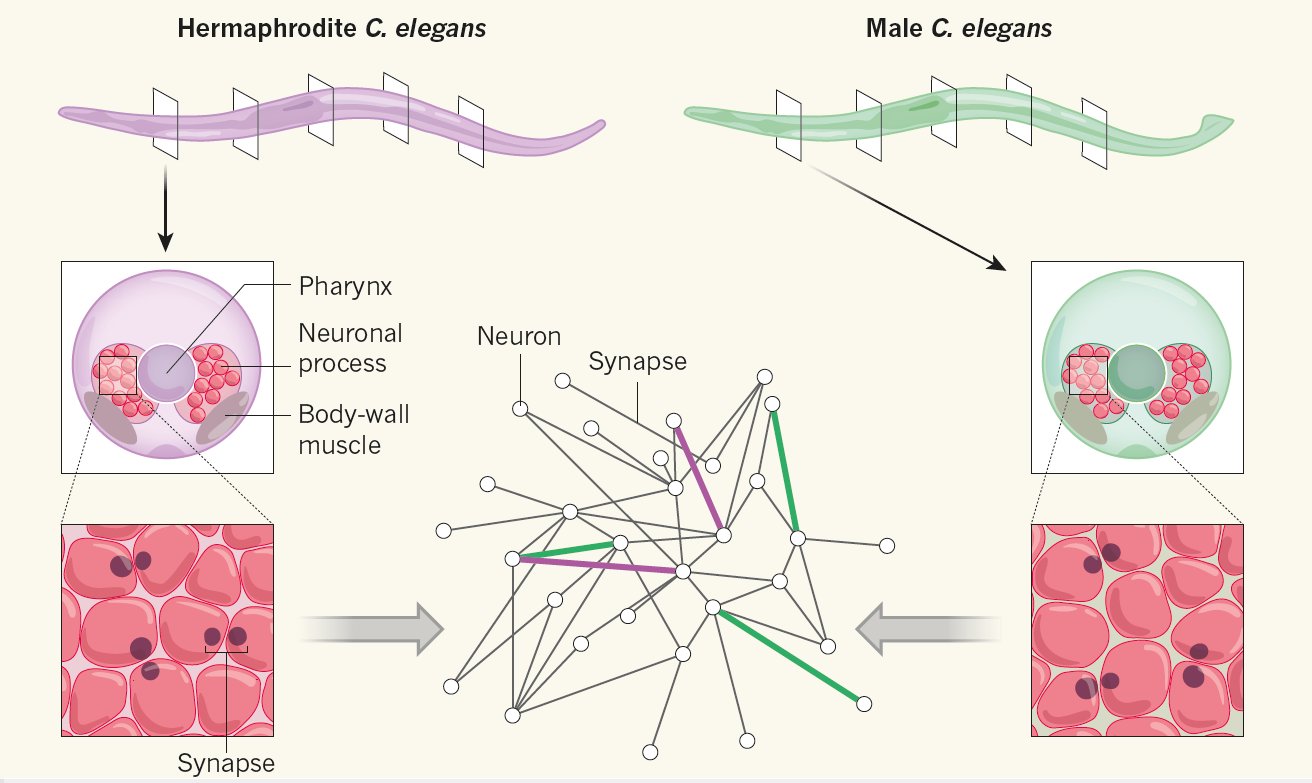
\includegraphics[width=\imsize]{conectoma.png}
	\caption[Mapeo del conectoma  del gusano.  ]{ Mapeo del conectoma  del gusano.  Cook et al. \protect\cite{cook_whole-animal_2019}  llevaron a cabo el mapeo de los sistemas nerviosos completos del gusano nematodo Caenorhabditis elegans, tanto del sexo hermafrodita como del macho, con una asombrosa resolución subcelular.   En la parte superior de la figura, se aprecia el uso de decenas de miles de secciones seriadas que abarcan la mayor parte del cuerpo del gusano adulto. Se obtuvieron imágenes de microscopía en baja y alta resolución de estas secciones, lo que permitió revelar la anatomía de una sección típica, incluyendo los procesos neuronales y las conexiones sinápticas. Estas imágenes sirvieron de base para la construcción de un conectoma, un mapa que visualiza las conexiones entre todas las neuronas. En el centro de la figura, se muestra una versión simplificada de este conectoma. La mayoría de las conexiones se encuentran en ambos sexos (indicadas en gris), aunque algunas son exclusivas de un sexo o presentan una mayor fortaleza en uno que en el otro (resaltadas en púrpura y verde).   (Adaptada de \protect\cite{portman_neural_2019}).}\label{fig:conectoma}
\end{figure}


\subsection{Métodos de Reconstrucción de Conectomas}

La reconstrucción de conectomas se ha beneficiado de diversas metodologías. La microscopía electrónica ha permitido la reconstrucción a nivel sináptico, mientras que la combinación de técnicas de inyección de trazadores con imágenes ópticas de tomografía seriada de alto rendimiento ha posibilitado la reconstrucción de alta resolución en ratones. Además, la recopilación sistemática de datos de una gran cantidad de experimentos de trazado ha dado como resultado matrices de consenso que condensan las conexiones cerebrales en gatos, monos y ratas. Los avances en técnicas de resonancia magnética de difusión in vivo están haciendo que sea cada vez más factible reconstruir conectomas a macroescala en cerebros individuales de grandes simios y humanos. Con el desarrollo de técnicas como CLARITY y la Imagen de Luz Polarizada en 3D (3D-PLI), es probable que se obtengan reconstrucciones sin precedentes de la conectividad del conectoma en animales y humanos en el futuro \cite{heuvel_comparative_2016}.


\subsection{Conectoma de C. elegans Completo (Cook et al., 2019)}

Hasta el año 2019, el conectoma más completo se basaba en la reconstrucción realizada por White et al. \cite{white_structure_1997}. No obstante, es fundamental tener en cuenta que este conectoma se limitaba al sexo hermafrodita, lo que generaba incertidumbre acerca de posibles diferencias en el cableado entre sexos.  Además, la construcción manual del conectoma original planteaba inquietudes sobre la precisión de los datos. Para abordar estos desafíos, Cook et al. \cite{cook_whole-animal_2019} desarrollaron un software especializado que permitió la reconstrucción del conectoma del macho adulto de C. elegans, una región que alberga circuitos exclusivos de este sexo. Posteriormente, Cook et al. \cite{cook_whole-animal_2019} informaron sobre la reconstrucción del conectoma masculino en su totalidad, incluyendo el anillo nervioso, una región crucial para el procesamiento de información en el gusano. Además, los autores emprendieron la tarea de reconstruir completamente el conectoma hermafrodita desde cero, aprovechando su software para reanalizar las microfotografías originales de la década de 1980. 

La \Cref{fig:conectomaa} presenta el conectoma de ambos sexos. Estos nuevos conectomas aportan una riqueza de información que promete avanzar significativamente en la comprensión del campo. Mientras que los conectomas originales simplemente indicaban la presencia de sinapsis, Cook et al. [16] proporcionaron información más detallada, que incluye la ubicación física y el peso de cada sinapsis, un indicador indirecto de la fuerza de la conexión en función de su tamaño físico. Este nivel de detalle permitirá análisis y modelados más sofisticados de la función de los circuitos neuronales. A través de su software, los investigadores también identificaron miles de conexiones previamente pasadas por alto en el hermafrodita. 

Utilizando herramientas de teoría de redes, introdujeron nuevas clasificaciones de grupos de neuronas en función de sus conexiones. Al comparar sus reconstrucciones de los lados izquierdo y derecho del gusano, que son en gran medida simétricos, los autores determinaron una alta precisión en los datos del conectoma. Los nuevos conectomas además incorporan detalles inéditos sobre las salidas del sistema nervioso, incluyendo conexiones previamente desconocidas con el intestino, la epidermis y la gónada masculina, lo cual inspira nuevas perspectivas en la fisiología y el metabolismo del gusano. También se identificó una complejidad inesperada en el control de los músculos del cuerpo \cite{portman_neural_2019}. 

A pesar de estos avances, el estudio presenta ciertas limitaciones, como la incertidumbre respecto a la cantidad de variabilidad entre individuos, la falta de claridad en cuanto a cómo la fuerza de una conexión se relaciona con su tamaño físico y el desafío de inferir la función únicamente a partir de la estructura del conectoma. En resumen, los conectomas representan mapas de posibilidades y, aunque revelan la totalidad de las sinapsis, proporcionan escasas pistas sobre cuáles están activas en un momento dado. 


 \begin{figure}[h!]
	\centering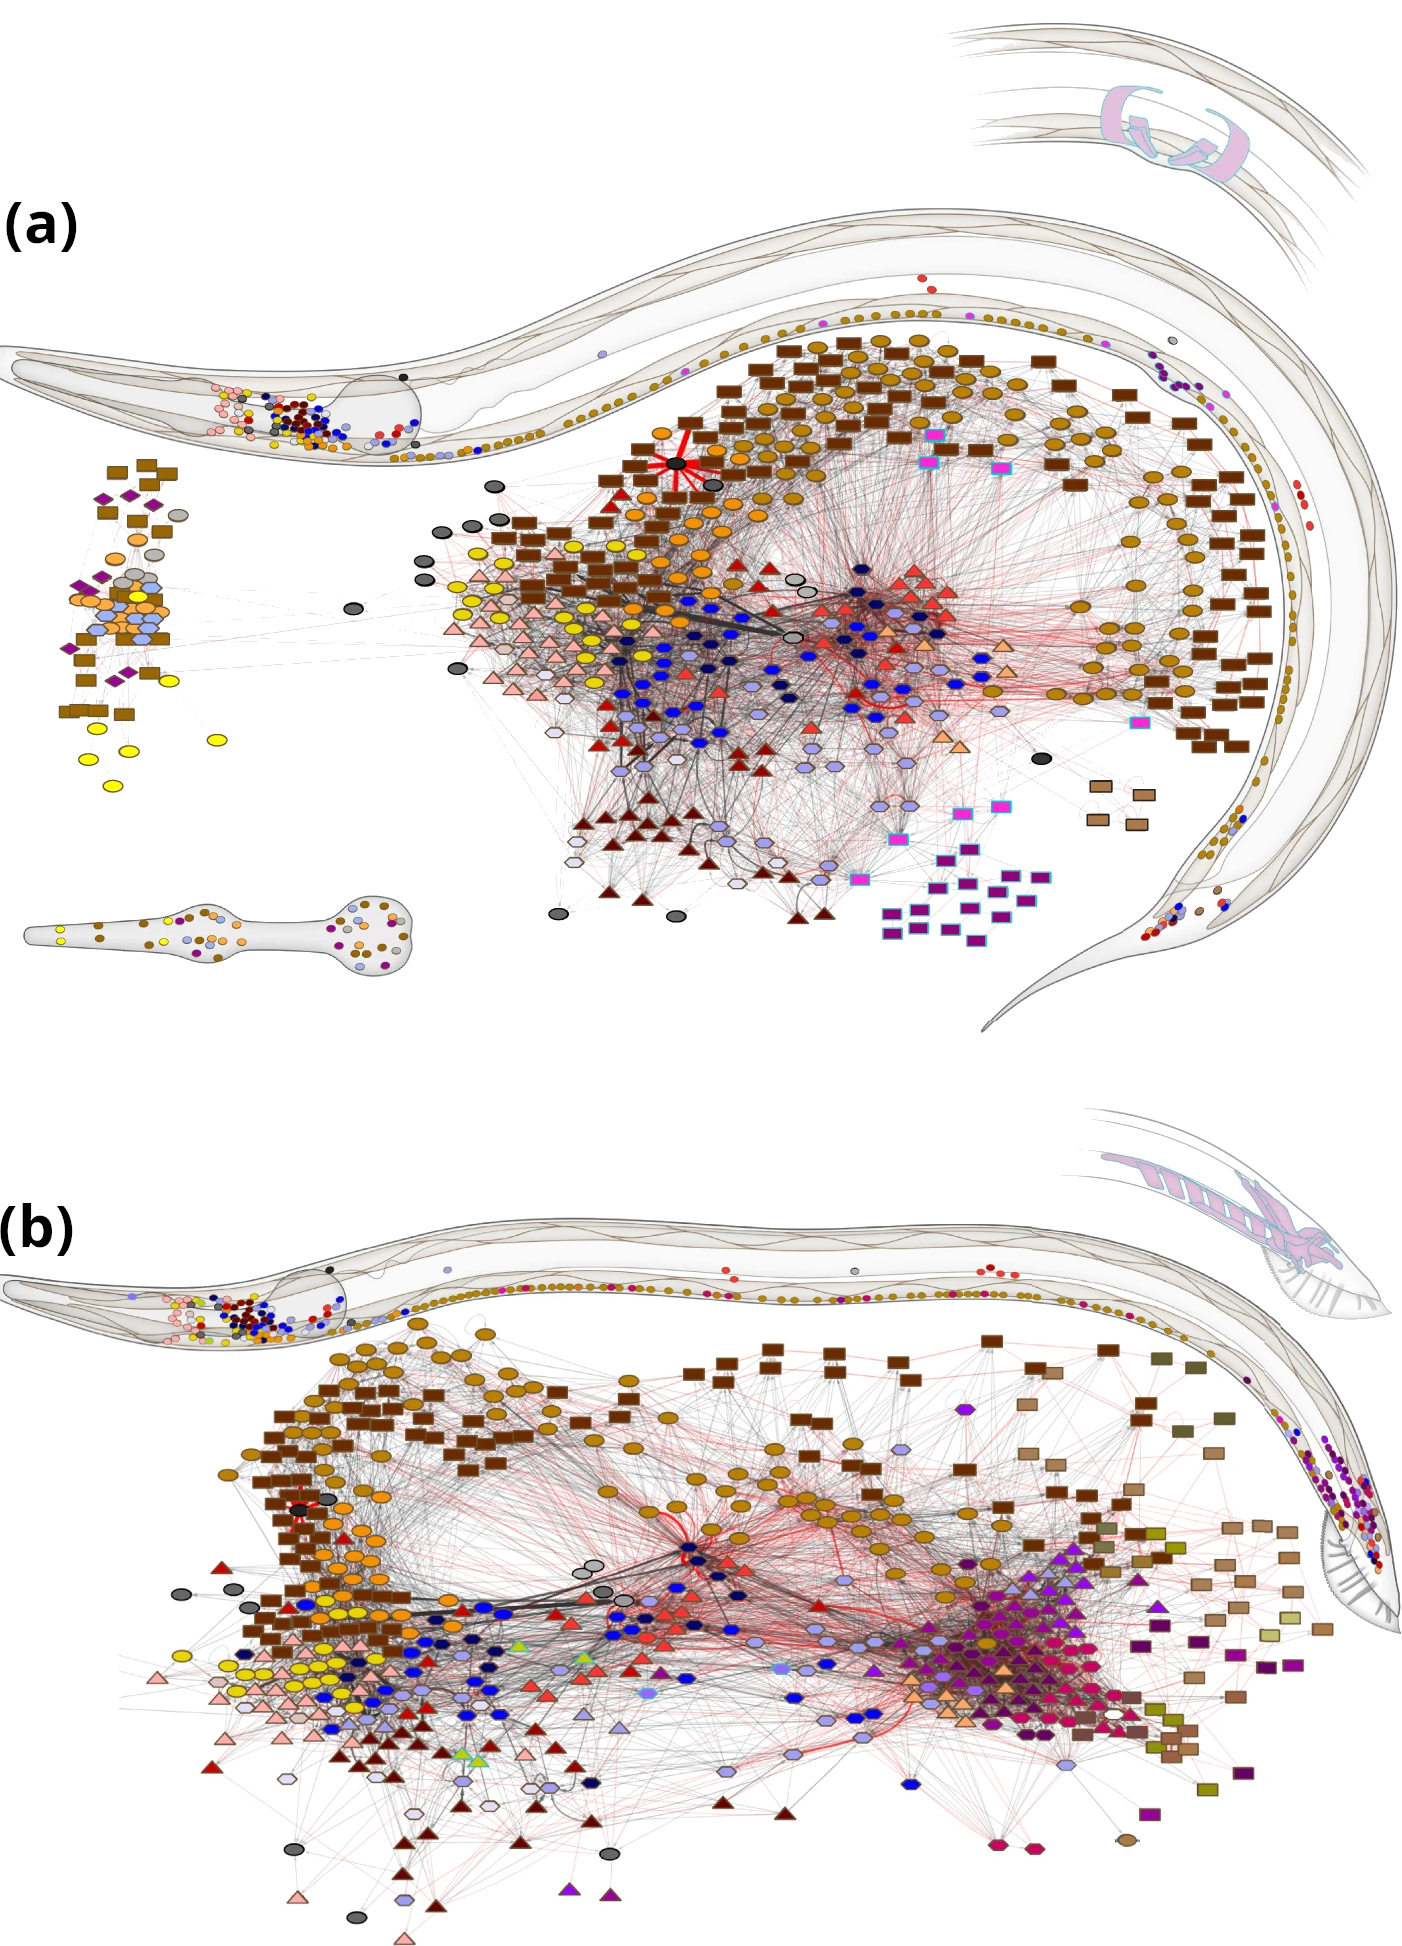
\includegraphics[width=\imsize]{conectoma_b.png}
	\caption[Conectividad del Sistema Nervioso  de C. elegans. Adultos.]{ Conectividad del Sistema Nervioso  de C. elegans. Adultos. (a) Representación del hermafrodita adulto. (b) Representación del macho adulto. En los cuadros ubicados en la esquina superior derecha de cada imagen, se resalta la ubicación de los músculos sexuales. Los diagramas de los gusanos indican la posición de los núcleos celulares.  En los grafos, la disposición de los vértices se basa en un algoritmo que agrupa las células altamente conectadas. Los bordes dirigidos, representados por flechas negras, indican las sinapsis químicas, mientras que los bordes no dirigidos, marcados con líneas rojas, representan las conexiones gap junctional. El ancho y la transparencia de las líneas denotan la fuerza de las conexiones. Una clave única se emplea para interpretar los diagramas de la red: triángulos para las neuronas sensoriales, hexágonos para las interneuronas, óvalos o círculos para las neuronas motoras, y rectángulos para los músculos. Los colores cumplen distintas funciones: varios tonos de rojo identifican las categorías de neuronas sensoriales según la modalidad y similitud de conectividad; tonos de azul señalan las categorías de interneuronas de acuerdo con su asignación a una capa específica; las clases de neuronas motoras se representan en varios tonos de amarillo y naranja, como se describe en el texto; por último, los órganos terminales no musculares se destacan en blanco, gris o negro.  (Adaptada de \protect\cite{cook_whole-animal_2019}).}\label{fig:conectomaa}
\end{figure}


\subsubsection{Matrices de adyacencia}


La matriz de adyacencia, que describe la estructura del sistema nervioso como un grafo de conectividad, se abstrae a partir de los mapas neuronales como una matriz de adyacencia con pesos que cuantifican la cantidad total de conectividad física entre cada par de células y se obtienen a partir de la suma de los tamaños de las conexiones sinápticas, que a menudo consisten en múltiples sinapsis. Dado que gran parte del sistema nervioso de C. elegans está compuesto por procesos simples y no ramificados que se encuentran en haces longitudinales donde establecen sinapsis de paso, se utilizó el método de anotación para estimar el tamaño de la mayoría de las sinapsis, contando las secciones atravesadas por la estructura sináptica. La cantidad de secciones varía entre 1 y 23 para las sinapsis químicas en el hermafrodita y entre 1 y 41 en el macho, mientras que para las sinapsis eléctricas oscila entre 1 y 20 en el hermafrodita y entre 1 y 30 en el macho. El grafo del conectoma hermafrodita consta de 460 nodos, que comprenden 302 neuronas, 132 músculos y 26 órganos terminales no musculares, mientras que el grafo del macho tiene 579 nodos, compuestos por 385 neuronas, 155 músculos y 39 órganos terminales no musculares. Estos grafos incluyen respectivamente 4.887 aristas químicas (con direccionalidad) y 1.447 aristas de unión en hendidura (sin direccionalidad) en el hermafrodita, y 5.315 químicas y 1.755 de unión en hendidura en el macho. A pesar de ser grafos dispersos, representan el 3,2 \% y el 2,4 \% de todas las aristas posibles en el caso del hermafrodita y el macho, respectivamente. Si se consideran todas las aristas sin direccionalidad en ambos sexos, se establece una conectividad débil, ya que existe al menos un camino que conecta cada par de nodos. La fracción de conectividad física debida a las uniones en hendidura varía ampliamente entre las clases de neuronas, fluctuando entre más del 90 \% y menos del 5 \% para las interneuronas no faríngeas. Los grafos de conectividad bidimensionales generados mediante métodos computacionales revelan las rutas de flujo de la información sensorial, con un pequeño número de pasos sinápticos (generalmente entre 1 y 5) entre las neuronas sensoriales y los órganos terminales, lo que sugiere una naturaleza de red "feedforward". La disposición de los nodos en los grafos muestra similitudes notables con la neuroanatomía del gusano, lo que refleja un cableado eficiente, una característica común en los sistemas nerviosos, incluso en C. elegans \cite{cook_whole-animal_2019}. .



La matriz de adyacencia generada se encuentra disponible en archivos de Excel que describen cada sinapsis, sus propiedades y un identificador único. Este número de identificación puede ingresarse en la página de neuronas de WormWiring (\url{http://wormwiring.org/}), lo que permite la ubicación de la sinapsis en el mapa. Al hacer clic en la sinapsis en el mapa, se acceden a las microfotografías pertinentes para su visualización.



\section{ Registro a Gran Escala de la Actividad Neuronal en C. elegans}


En los apartados  previos, se ha abordado la caracterización de las conexiones neuronales desde un enfoque principalmente estructural. Aunque el conectoma estructural proporciona una visión esencial del sistema nervioso, su comprensión integral se ve limitada por esta perspectiva.  Sin embargo, en la búsqueda de una comprensión más integral, la neurociencia ha desarrollado enfoques innovadores que tratan de cerrar la brecha entre la estructura anatómica y la función de los circuitos neuronales.

Estos nuevos enfoques aprovechan indicadores fluorescentes de actividad neuronal, permitiendo la observación en tiempo real del flujo de señales a través del sistema nervioso de C. elegans mientras el organismo se encuentra en un estado de comportamiento libre. Esta dinámica actividad neuronal se superpone con el conectoma estructural, proporcionando así una ventana a cómo la estructura física influye en la función.

Este apartado se centra en exponer los experimentos más recientes que siguen esta línea de investigación. La neurociencia de sistemas ha experimentado una tendencia general hacia la obtención de una imagen más completa de la actividad neuronal en el cerebro. La grabación simultánea de poblaciones neuronales ha emergido como una técnica superior en comparación con las grabaciones secuenciales de unidades individuales. No solo permite la captura de información de múltiples neuronas en un período de tiempo más corto, sino que también proporciona la oportunidad de realizar descubrimientos inesperados gracias a la simultaneidad de las grabaciones.


El registro de la actividad neuronal en todo el cerebro es atractivo debido a su potencial de ofrecer una visión exhaustiva. La idea subyacente es que el registro de la actividad de todas las neuronas de un organismo con un mapeo detallado de las conexiones neuronales podría eliminar las restricciones convencionales que dificultan la comprensión de fenómenos neuronales específicos. Esto reduciría la posibilidad de atribuir observaciones no explicadas a neuronas no registradas o conexiones no identificadas, lo que contribuye a la mejora de los modelos y al refinamiento de nuestra comprensión en este campo.


Aunque en organismos con sistemas nerviosos más complejos, como los vertebrados, esta perspectiva presenta desafíos sustanciales debido al aumento en la dimensionalidad de los datos, en organismos más pequeños, como C. elegans, se han logrado mediciones de actividad cerebral casi completa a nivel de una sola célula. Estos logros prometen brindar conceptos que pueden extrapolarse a redes de mayor tamaño.

Uno de los sujetos de estudio más exitosos en esta área es la larva del pez cebra. Investigadores han observado el cerebro de estos animales mientras llevan a cabo la natación ficticia y se mantienen inmovilizados en agar. Este avance se ha logrado mediante técnicas de microscopía de lámina de luz, lo que ha permitido la identificación de diversos patrones de actividad y sus relaciones en contextos de comportamiento. Además, otro organismo modelo que se presta bien a este tipo de análisis es el nematodo C. elegans. 

Este organismo destaca, en particular, por su transparencia óptica, siendo el primero en el que se expresó la proteína verde fluorescente (GFP). Este hito desencadenó una revolución en la imagenología biológica en tiempo real. Más recientemente, los investigadores han realizado trabajos pioneros para monitorear la actividad neuronal y muscular en gusanos a través de la fluorescencia de indicadores de calcio. Varios laboratorios han tenido éxito en la captura de imágenes de todo el cerebro de C. elegans \cite{kaplan_nested_2020,kato_global_2015,yemini_neuropal_2021}, demostrando que las actividades neuronales globales generan una diversidad de estados en los que se representan comportamientos característicos, como avanzar, retroceder y girar \cite{kato_global_2015}. Además, se han obtenido imágenes de todo el cerebro en animales en movimiento libre, lo que ha permitido la identificación de actividades relacionadas con comportamientos específicos \cite{kaplan_nested_2020}.


En este trabajo, nuestro enfoque se centrará principalmente en C. elegans. A pesar de las diferencias fundamentales en el sistema nervioso de C. elegans en comparación con los vertebrados, como la predominancia de potenciales graduales de variación lenta en lugar de los potenciales de acción rápidos comunes en vertebrados, el estudio del procesamiento de información, los patrones de circuitos y la relación entre la estructura y la función del sistema nervioso prometen proporcionar información valiosa que puede enriquecer nuestra comprensión, incluso a nivel inter-especie \cite{randi_measuring_2020}.


\subsection{Mapeo de la Actividad Neuronal Asociada a la Locomoción}\label{sec:kato}


En el afán de explorar cómo los sistemas nerviosos codifican, organizan y secuencian los comportamientos, Kato et al. (2015) realizaron una investigación que arrojó luz sobre la dinámica neuronal que subyace a la locomoción en C. elegans. Mediante la combinación de tecnologías innovadoras, incluyendo la obtención de imágenes de casi la totalidad del sistema nervioso con resolución celular, los autores presentan evidencia que sugiere que los comandos motores en C. elegans se encuentran representados por amplias poblaciones de neuronas con dinámicas cíclicas. Esta observación no solo extiende nuestras percepciones, sino que también refuerza observaciones previas relacionadas con una variedad de comportamientos que abarcan desde la digestión hasta la toma de decisiones en una amplia gama de organismos, desde sanguijuelas hasta primates \cite{branson_imaging_2015}.

El enfoque utilizado por Kato et al. implicó la obtención de imágenes de la actividad neuronal de aproximadamente 100 neuronas en los sistemas nerviosos de gusanos mantenidos en reposo en un canal angosto. Este proceso hizo uso del indicador de calcio genéticamente codificado GCAMP, el cual emite fluorescencia verde en las neuronas activas. Las imágenes se capturaron mediante un microscopio confocal comercial de alta velocidad, lo que permitió la adquisición de imágenes volumétricas de todo el cerebro a intervalos de un tercio de segundo. Este enfoque proporcionó una resolución de una sola neurona en la mayoría del sistema nervioso y, cuando se complementó con el profundo conocimiento previo de la anatomía neuronal de C. elegans, permitió la identificación de la gran mayoría de las neuronas.

A pesar de la inmovilidad de los gusanos, sus sistemas nerviosos mostraron actividad neuronal durante períodos prolongados, de aproximadamente 20 minutos por individuo. Los datos resultantes, que representan series temporales de 100 dimensiones describiendo la actividad neuronal (una dimensión por cada célula), son intrincados y requieren un análisis avanzado. Kato et al. emplearon el análisis de componentes principales (PCA) para reducir los datos de alta dimensión a trayectorias bidimensionales o tridimensionales (\Cref{fig:kato1}A). Estas representaciones simplificadas capturaron de manera más accesible la estructura de las poblaciones neuronales, revelando trayectorias de actividad neuronal que seguían patrones cíclicos y altamente repetitivos. Dichos patrones estereotipados de actividad neuronal se sucedían en secuencia, de tal manera que el ciclo se repetía. Además, se observó que múltiples neuronas contribuían a esta representación, lo que sugiere que estas dinámicas neuronales, a pesar de ser reducidas a unas pocas dimensiones, estaban distribuidas en una amplia variedad de neuronas.


 \begin{figure}[h!]
	\centering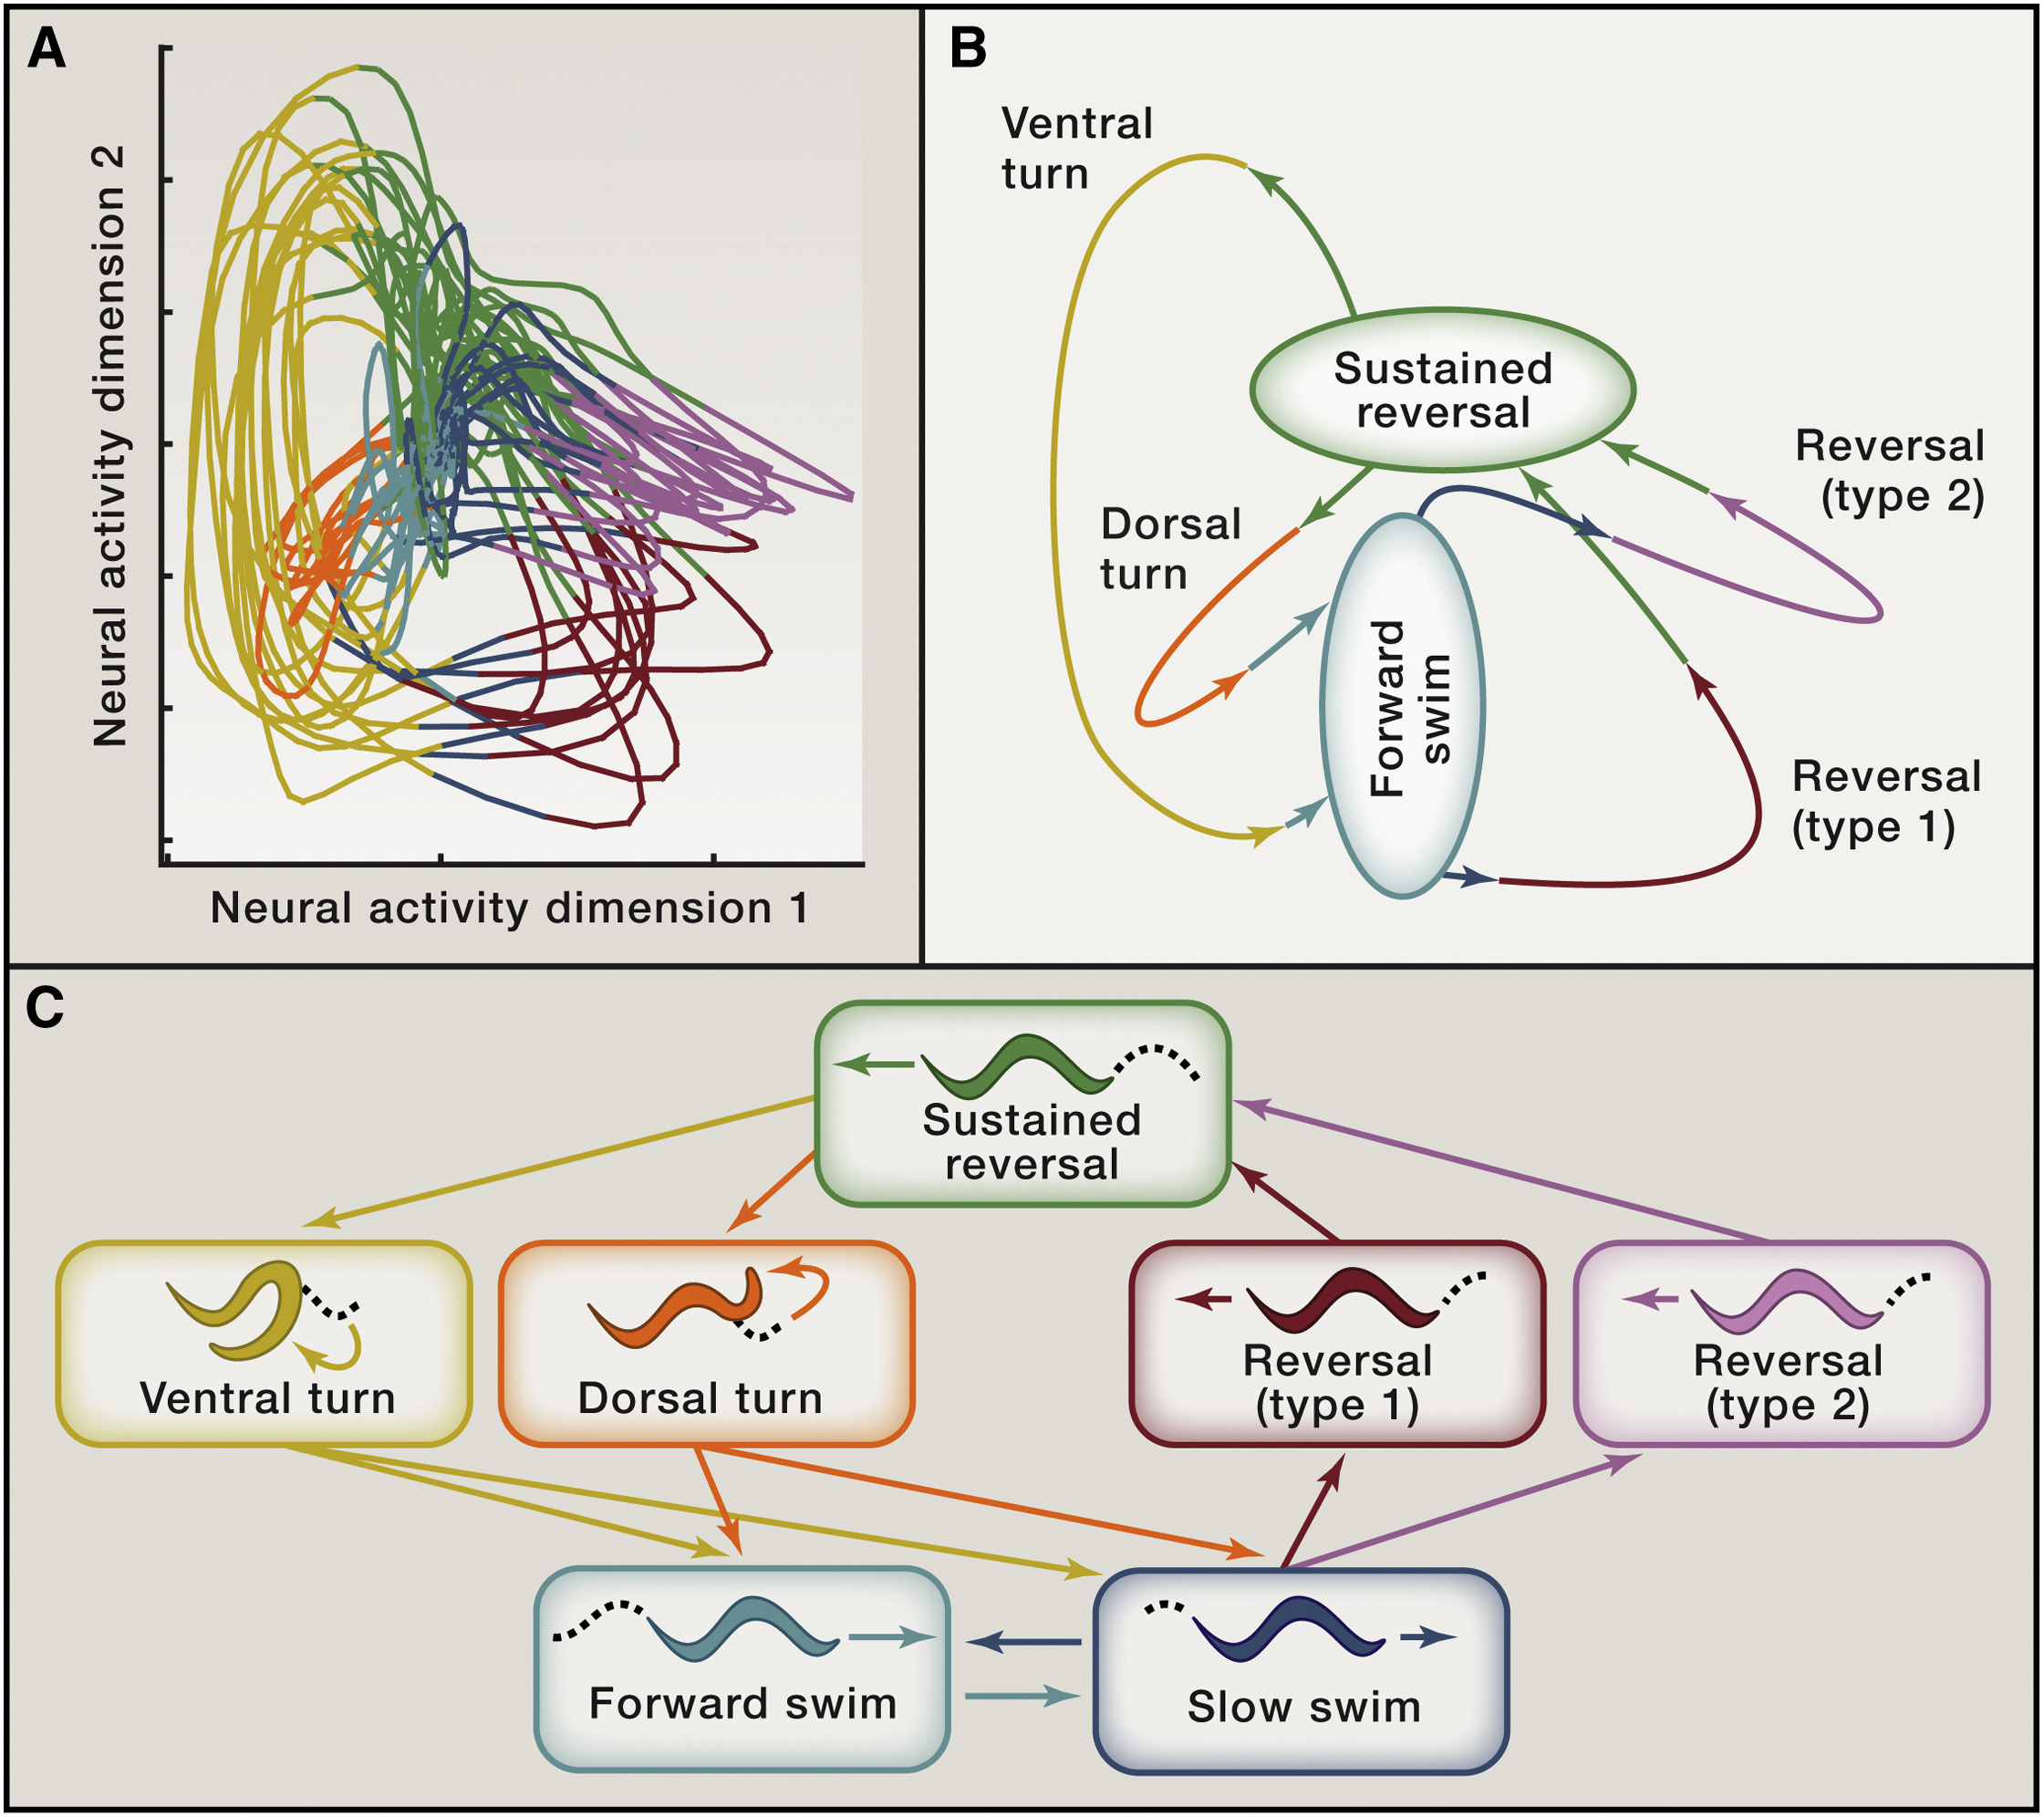
\includegraphics[width=\imsize]{kato_2.jpg}
	\caption[Representación de la Trayectoria de la Actividad Neuronal en C. elegans.]{ Representación de la Trayectoria de la Actividad Neuronal en C. elegans. (A) La trayectoria que ilustra la actividad neuronal, obtenida mediante imágenes que abarcan casi la totalidad del cerebro con una resolución celular en C. elegans, se proyecta en los dos primeros componentes principales. Esta dinámica presenta un patrón cíclico y estereotipado, donde la variación en el color identifica a qué grupo específico pertenece cada segmento de actividad neuronal. (B) En el espacio de actividad neuronal, se destacan regiones que se correlacionan con comportamientos específicos, indicando la relación entre la actividad neuronal y la locomoción observada. (C) Se presenta un diagrama de transición de estados que captura la dinámica de locomoción en C. elegans en paralelo con la actividad neuronal destacada en (B). Este diagrama arroja luz sobre la conexión entre la actividad neuronal y los comportamientos locomotores del gusano. (Adaptada de \protect\cite{branson_imaging_2015}). }\label{fig:kato1}
\end{figure}


Para validar estos resultados, Kato et al. llevaron a cabo un segundo conjunto de experimentos en los que obtuvieron imágenes de la actividad neuronal en gusanos que se comportaban libremente, mientras observaban simultáneamente la locomoción. Sorprendentemente, los grupos en el espacio de trayectoria neuronal, definidos únicamente en función de la actividad neuronal, se correlacionaban con diferentes comportamientos de locomoción, como avanzar, retroceder, girar y detenerse.


Por lo tanto, se infiere que una parte sustancial de la actividad neuronal en C. elegans, incluso en condiciones de inmovilidad, codifica el estado locomotor ficticio. El flujo de actividad neuronal (\Cref{fig:kato1}B) presenta similitudes con un diagrama de transición de estados de comportamiento  (\Cref{fig:kato1}C), una representación comúnmente utilizada para visualizar los tipos y probabilidades de transiciones de comportamiento observadas. Un rasgo sorprendente de estos patrones de actividad neuronal es que son en gran medida autogenerados. En conjunto, estos hallazgos sugieren que una parte sustancial del cerebro del gusano oscila constantemente entre estados que, cuando el animal se encuentra en movimiento libre, inducen distintos comportamientos de locomoción. La información sensorial modula las probabilidades de entrar y salir de estos estados, lo que podría explicar la variabilidad observada en el comportamiento de locomoción de C. elegans.




\subsection{Implementación Neural de Jerarquías Conductuales}\label{sec:kaplan}


La conducta es una secuencia de acciones ordenadas que los organismos llevan a cabo en el tiempo para interactuar con su entorno. Varias disciplinas, como la etología, la psicología y la neurociencia, han reconocido que muchos comportamientos, tanto innatos como adquiridos, presentan una estructura jerárquica que abarca múltiples niveles. Estos niveles van desde objetivos generales y estados conductuales hasta secuencias de acciones, subtareas y elementos motores específicos. La neurociencia contemporánea se enfrenta al desafío de profundizar en la comprensión de cómo el sistema nervioso controla y coordina estos niveles jerárquicos de comportamiento.

Para abordar este desafío, Kaplan et al. \cite{kaplan_nested_2020} llevaron a cabo una serie de experimentos que proporcionan información valiosa sobre la jerarquía espaciotemporal de dinámicas neuronales que abarcan todo el cerebro y la periferia de C. elegans durante su comportamiento locomotor  \cite{hollon_neural_2020}. Los mecanismos detallados de los circuitos descubiertos arrojan luz sobre cómo el sistema nervioso puede generar múltiples niveles de jerarquía conductual y coordinar sus interacciones para producir la salida motora en diferentes escalas temporales.


En su estudio, Kaplan et al.   caracterizaron por primera vez la locomoción en C. elegans como un proceso compuesto por varios niveles dentro de una jerarquía conductual (ver \Cref{fig:kaplan1}).  En el nivel superior, los gusanos se desplazan hacia adelante o hacia atrás, alterando su dirección de manera intermitente, aproximadamente cada 20 segundos. En el nivel intermedio, se encuentran las ondulaciones que se propagan a lo largo del cuerpo del gusano para impulsar su avance. Estas \textquote{curvas propagadas } inician su movimiento de la cabeza a la cola durante la locomoción hacia adelante y de la cola a la cabeza durante la locomoción hacia atrás, con un período de alrededor de 2 segundos. El nivel más bajo de la jerarquía conductual implica movimientos rápidos de la cabeza que ocasionalmente realizan los gusanos y que no se propagan completamente hasta la cola. Estos \textquote{lanzamientos de cabeza} de 1 segundo ocurren exclusivamente durante la locomoción hacia adelante, y su dirección está estrictamente ligada al ángulo de la última curva propagada, con lanzamientos de cabeza dorsales después de curvas dorsales y lanzamientos de cabeza ventrales después de curvas ventrales.




\begin{figure}[h!]
	\centering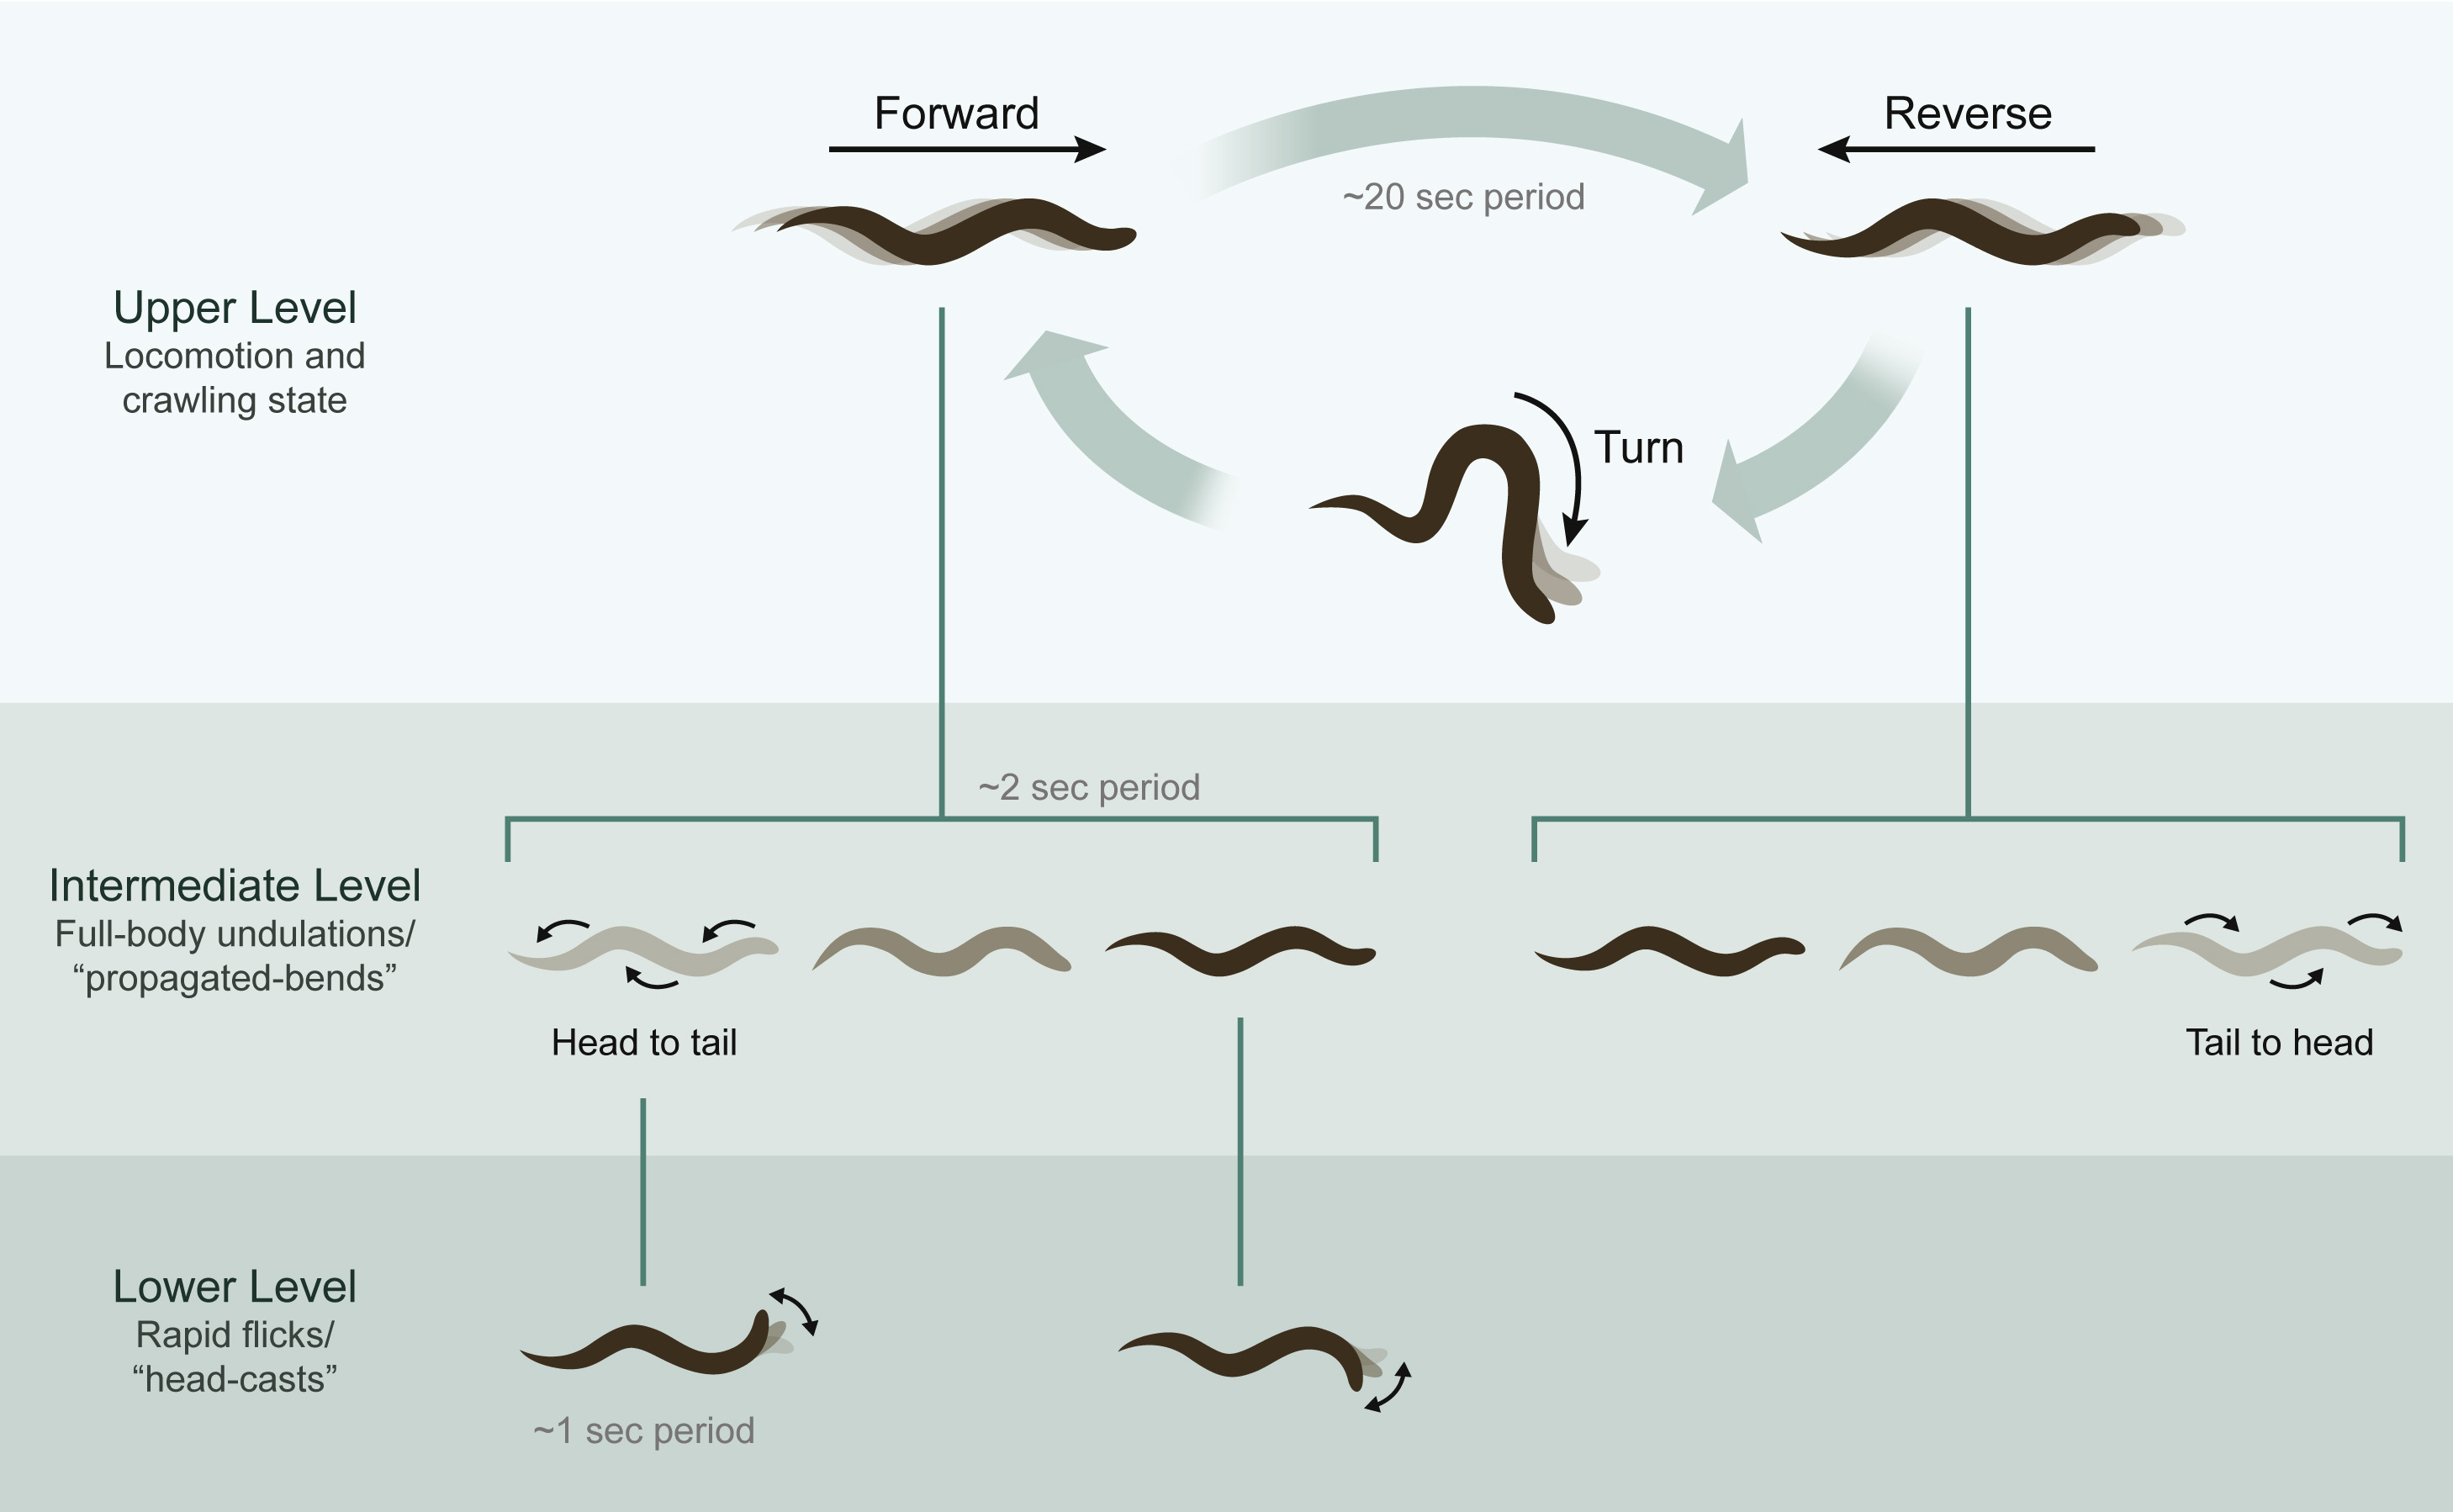
\includegraphics[width=\imsize]{kaplan1.jpg}
	\caption[Jerarquía Conductual en la Locomoción de C. elegans.]{ Jerarquía Conductual en la Locomoción de C. elegans. Esta representación visual nos permite observar cómo el comportamiento locomotor de C. elegans se organiza en distintos niveles jerárquicos, cada uno operando en escalas de tiempo específicas. La jerarquía conductual se refleja en la diferente duración de los comportamientos en C. elegans, lo que se traduce en distintas escalas de tiempo para cada nivel.	 (Figura adaptada de \protect\cite{hollon_neural_2020}). }\label{fig:kaplan1}
\end{figure}


Los experimentos de manipulación realizados por Kaplan et al.  indican que los diferentes niveles de la jerarquía de la locomoción en C. elegans están organizados de manera funcional jerárquica, con los niveles superiores ejerciendo influencia sobre los niveles inferiores, pero con una influencia limitada en la dirección opuesta. Es importante destacar que los patrones de actividad neuronal oscilatoria y su anidamiento jerárquico se mantuvieron incluso en animales físicamente inmovilizados, aunque a frecuencias generales más bajas, lo que sugiere que estas dinámicas rítmicas pueden persistir en gran medida independientemente de la retroalimentación propioceptiva. En conjunto, estos resultados respaldan la idea de que la organización jerárquica del comportamiento podría derivar, al menos en parte, de una organización intrínseca jerárquica de los circuitos de control motor.


\subsection{NeuroPAL: Un Avance en la Identificación Neuronal en C. elegans}


La adquisición y análisis de conjuntos de datos neuronales en C. elegans, como se ha detallado anteriormente, se han enfrentado a desafíos considerables, principalmente relacionados con la identificación precisa de neuronas en las imágenes microscópicas de estos organismos. En las investigaciones neurocientíficas con C. elegans, es común utilizar promotores de genes específicos para expresar la proteína verde fluorescente (GFP) con el propósito de determinar qué neuronas expresan dicho gen. Sin embargo, este enfoque se ha visto limitado por la identificación precisa de neuronas, ya que en muchas ocasiones, las neuronas adyacentes presentan morfologías similares y/o posiciones variables, lo que compromete la fiabilidad del proceso.

Para abordar este desafío, Yemini et al. \cite{yemini_neuropal_2021} han desarrollado la innovadora herramienta denominada \gls{NeuroPAL} (Neuronal Polychromatic Atlas of Landmarks).    El transgén NeuroPAL permite la expresión de diferentes combinaciones de cuatro proteínas fluorescentes distintas de la GFP en diversas neuronas de C. elegans. Este enfoque permite que las neuronas cercanas se iluminen con colores diferentes, lo que facilita su identificación de manera fiable (consulte la \Cref{fig:neuropal}). Las cuatro proteínas fluorescentes utilizadas en el NeuroPAL poseen espectros de excitación/emisión que las hacen fácilmente distinguibles entre sí y de la GFP. Como resultado, a través de sencillos cruces genéticos, es posible generar animales que portan tanto un transgén GFP como un transgén NeuroPAL, lo que, en principio, permite la identificación precisa de las neuronas que expresan GFP \cite{santiago_using_2022}.
 
La introducción de NeuroPAL ha supuesto un avance significativo en la identificación de neuronas en C. elegans, allanando el camino para un análisis más preciso y confiable de los datos neuronales. Esto, a su vez, ha contribuido al mejor entendimiento de la neurobiología de este modelo, fortaleciendo las bases para futuras investigaciones en este campo de estudio.

\begin{figure}[h!]
	\centering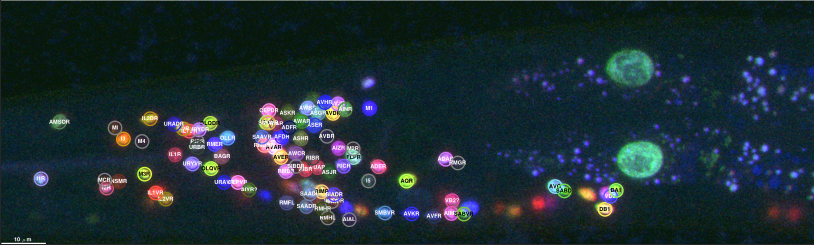
\includegraphics[width=\imsize]{neuropal.png}
	\caption[Visualización de la Actividad Neuronal en la Cabeza con NeuroPAL.	]{ Visualización de la Actividad Neuronal en la Cabeza con NeuroPAL.}\label{fig:neuropal}
\end{figure}


\section{Modelo de Procesamiento Sensoriomotor en C. elegans: Una Perspectiva Distribuida y Dinámica}\label{sec:modelo}

En esta sección, se presenta un modelo presente en la literatura que aborda la cuestión de cómo, desde una perspectiva neurobiológica, C. elegans podría llevar a cabo el procesamiento sensoriomotor. El propósito de este modelo es abordar la carencia teórica existente al integrar coherentemente los resultados previamente descritos relacionados con las conexiones neuronales (conectoma), los circuitos con funciones específicas y la dinámica neuronal a nivel global.  Este marco teórico proporcionará una base sólida para comprender la interacción entre la dinámica neuronal, el conectoma y el comportamiento en nuestro modelo robótico.


En investigaciones recientes, se ha avanzado hacia una visión más completa de cómo el sistema nervioso del C. elegans podría llevar a cabo cálculos y tomar decisiones en respuesta a las señales sensoriales recibidas. Estudios previos postulaban que la información fluía de manera predominantemente segregada y directa desde los circuitos sensoriales hacia los motores. Además, se clasificaban a las neuronas motoras en categorías dirigidas hacia los músculos de la cabeza o del cuerpo, mientras se identificaban cinco interneuronas premotoras como puntos neurales centrales en la red, recibiendo múltiples entradas de los circuitos sensoriales y funcionando como un cuello de botella en la transmisión de señales hacia las neuronas motoras del cuerpo  \cite{gray_circuit_2005} .  Esto sugiere una estrategia secuencial en la que la información sensorial de múltiples señales se integra en un grupo de interneuronas de la primera capa, que luego transmiten esta información, posiblemente transformada, a un grupo de interneuronas de la segunda capa. Estas últimas interconectan finalmente con las neuronas motoras de la cabeza y las interneuronas premotoras centrales para dirigir el comportamiento. La secuencia de procesamiento sensoriomotor se ilustra en la \Cref{fig:computosistema}.


\begin{figure}[h!]
	\centering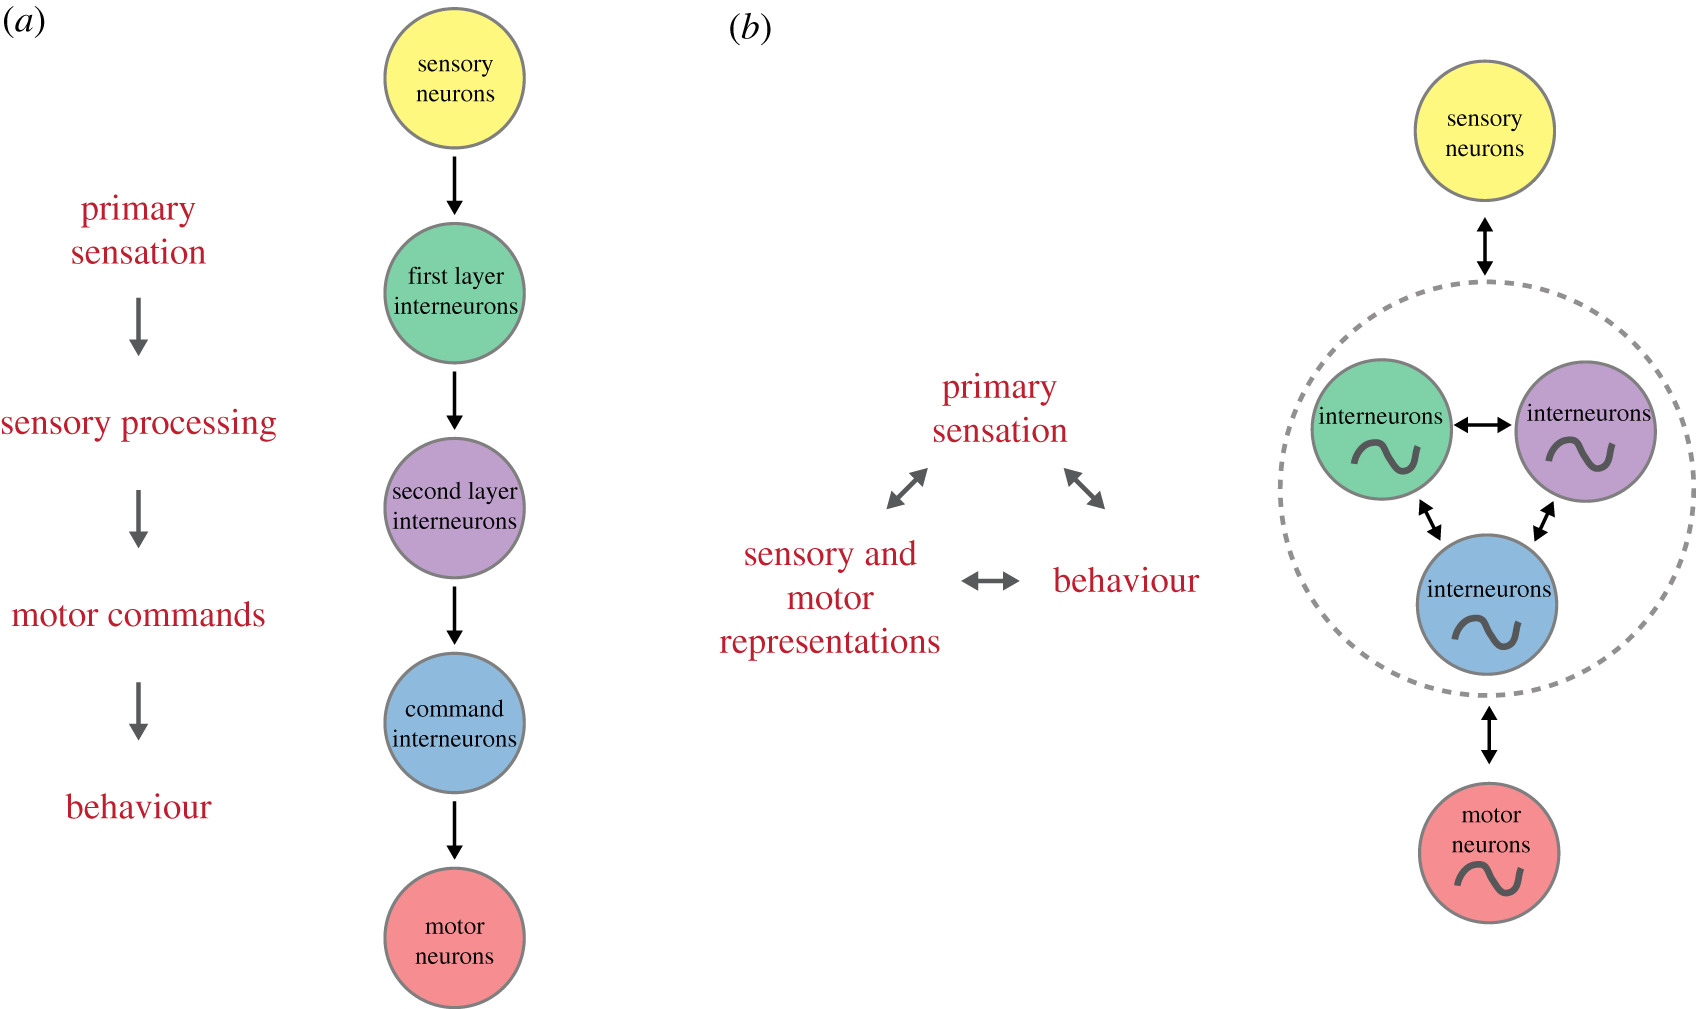
\includegraphics[width=\imsize]{sensioral.jpg}
	\caption[ Dos Modelos Contrastantes del Flujo Sensoriomotor en C. elegans.]{ Dos Modelos Contrastantes del Flujo Sensoriomotor en C. elegans. Dentro del contexto del procesamiento sensoriomotor en C. elegans, se contrastan dos modelos fundamentales  que representan enfoques diferentes para comprender cómo este organismo realiza estas funciones cruciales. El modelo (a), que denominamos \textquote{Modelos Secuenciales Segregados}, sugiere que la transformación de las representaciones sensoriales a las motoras sigue principalmente una ruta de alimentación directa y funcionalmente segregada a nivel de circuitos neuronales. En este enfoque, los cálculos se llevan a cabo en un orden temporal secuencial, con una clara distinción entre las etapas sensoriales y motoras. En contraste, el modelo (b), que llamaremos \textquote{Modelos Distribuidos}, es más consistente con los datos experimentales y propone una representación distribuida de las variables sensoriales y motoras a través de los circuitos neuronales. En este enfoque, se enfatiza la retroalimentación entre la mayoría de los elementos del sistema como una propiedad esencial. Las entradas sensoriales se integran de manera dinámica con la actividad interna de los circuitos neuronales, lo que permite que los cálculos se realicen de manera concurrente. En este modelo, las interacciones recíprocas dinámicas entre el cerebro, el cuerpo y el entorno son fundamentales para el procesamiento sensoriomotor.	  (Adaptada de \protect\cite{kaplan_sensorimotor_2018} ).}\label{fig:computosistema}
\end{figure}


No obstante, investigaciones más recientes han revelado una dinámica inesperada en la actividad de estas interneuronas. En lugar de actuar únicamente como mediadoras de la información sensorial, se ha observado que desempeñan un papel activo en la generación de comandos motores. Este hallazgo se sustenta en observaciones de animales inmovilizados, donde las actividades de las interneuronas se correlacionan de manera dinámica y coordinada. Las neuronas coactivas en estas grabaciones mantienen su actividad en un mismo estado motor, con escasas excepciones.

Kaplan et al. \cite{kaplan_sensorimotor_2018} postulan que el sistema nervioso del C. elegans se comprende mejor como un sistema distribuido y dinámico diseñado para generar comportamiento adaptativo. Esta red distribuida recibe entradas de neuronas sensoriales y ajusta su dinámica para la toma de decisiones. La  \Cref{fig:computosistema}B ilustra este procesamiento neuronal distribuido y dinámico. Los comandos motores se condensan eficientemente en el denominado colector de atractores, que representa una representación de baja dimensión de la actividad neuronal de alta dimensión, como se detalló previamente. Este colector se caracteriza por la participación de un gran número de neuronas, fuertes correlaciones y anti-correlaciones entre ellas, y una repetición cíclica de los estados de actividad de la red que involucra de manera consistente las mismas clases de neuronas en cada ciclo \cite{kato_global_2015}.


Un aspecto relevante es la suavidad del colector de atractores a nivel de la población neuronal en C. elegans, lo que implica una transición gradual en la actividad de la red (ver \Cref{fig:kato1}A). Esta característica es fundamental para ajustar las métricas del movimiento al cambiar entre diferentes patrones locomotores, similar a cómo se reduce gradualmente la velocidad de un vehículo antes de cambiar a la marcha atrás.

Para evaluar la hipótesis de codificación poblacional, se han desarrollado métodos computacionales avanzados \cite{elsayed_structure_2017}. Además, se espera que la obtención de imágenes del cerebro completo de gusanos en movimiento libre revele correlaciones entre características poblacionales y comportamiento. En última instancia, la actividad altamente correlacionada y consistente de la red subyace en los comandos motores en el C. elegans.


Kaplan et al. \cite{kaplan_sensorimotor_2018} plantean que esta característica contribuye a la producción robusta del comportamiento, proporcionando una columna vertebral preconfigurada que persiste bajo flujos complejos de entradas multisensoriales, como las que los gusanos encuentran en su entorno natural del suelo. Las interneuronas desempeñan un papel crucial en este proceso debido a su conectividad excepcional, formando un \textquote{club rico} \cite{cook_whole-animal_2019}. Se sugiere que las probabilidades de transición en el colector de atractores dependen de la dinámica interna y de una función ponderada de las entradas sensoriales a las interneuronas, lo que explicaría la redundancia en los patrones de actividad relacionados con los comandos motores de diferentes interneuronas. Estas interneuronas no son redundantes, sino canales que diferencian las entradas en una red distribuida de comandos motores, influyendo en la dinámica en curso. 



\section{Integración de Modelos Robóticos y Neurobiología en C. elegans para la Investigación en Neuro-robótica}
\label{sec:neurorobot}
En esta apartado, se examinan  los modelos robóticos documentados en la literatura que buscan integrar los componentes previamente descritos: el conectoma, la función neuronal y el comportamiento del nematodo C. elegans.

En las últimas décadas, hemos sido testigos de avances significativos en el desarrollo de técnicas de inteligencia artificial (IA) para su aplicación en la robótica. A pesar de estos notables logros, subsisten limitaciones críticas en términos de generalización, aprendizaje y robustez en las soluciones implementadas. Para abordar estas limitaciones, ha emergido un enfoque prometedor: el estudio de sistemas biológicos. La comprensión de la relación entre el comportamiento y el procesamiento de la información en los circuitos neuronales constituye un desafío central en el campo de la neurociencia. Asimismo, esta comprensión puede sentar las bases para el desarrollo de algoritmos inspirados en los principios neuronales, con aplicaciones en la robótica \cite{norman-tenazas_worminator_2018}.


Un aspecto crítico para llevar a cabo la simulación de un sistema nervioso completo radica en la disponibilidad del conectoma de dicho sistema. Como se discutió en el \Cref{sec:conectoma} el conectoma se concibe convencionalmente como un grafo que constituye un objeto matemático compuesto por vértices, bordes dirigidos y atributos. La construcción de conectomas a partir de microscopía electrónica da lugar a gráficos anatómicos, donde los vértices representan neuronas individuales y los bordes representan conexiones sinápticas dirigidas.


La simulación de circuitos neuronales también conlleva la necesidad de una comprensión profunda de la dinámica neuronal y la neuromodulación, ya que diferentes dinámicas temporales neuronales pueden resultar en diferentes respuestas a partir del mismo conectoma subyacente. C. elegans, como organismo modelo, constituye una base sólida para la simulación en circuito cerrado del comportamiento. Su conectoma se caracteriza con gran detalle, si bien persisten incógnitas en relación a la dinámica neuronal y al papel de la neuromodulación. A pesar de ello, se han propuesto circuitos neuronales que explican una variedad de comportamientos observables, como la retracción al tacto y la exploración de entornos \cite{bargmann_chemosensation_2006}.


En este contexto, el proyecto OpenWorm ha desarrollado una simulación detallada que abarca todas las células relevantes del nematodo C. elegans, involucradas en procesos de detección y actividad motora \cite{sarma_openworm_2018}. Estas simulaciones se basan en modelos que describen la dinámica de los canales neuronales.

Además, investigaciones recientes han comparado la respuesta de retracción al tacto del gusano con políticas de control óptimas \cite{lechner_worm-level_2017}, y se ha propuesto un modelo de Simulink del gusano que se fundamenta en modelos de un solo compartimento. Otro enfoque consiste en la implementación de simulaciones dinámicas del conectoma de C. elegans en plataformas físicas y robóticas. Estos estudios aplican principios computacionales neuronales inspirados en el comportamiento de C. elegans al control de robots, lo que permite la comparación entre algoritmos basados en la biología y enfoques convencionales. Un ejemplo de ello es una plataforma robótica que ha implementado una simulación de seis neuronas relacionadas con la quimiotaxis de C. elegans \cite{morse_robust_1998}, aunque no ha simulado todo el sistema nervioso del gusano.

Recientemente, Timothy Busbice \cite{Timothy_robot}  ha desarrollado un modelo de red neuronal utilizando el conectoma completo del nematodo C. elegans como sustrato (consultar Figura 2.11). Este modelo de red neuronal se ha empleado para el control de un vehículo robot. La actividad de las neuronas sensoriales se estimuló mediante lecturas de un sensor de posición, y las salidas de las neuronas motoras del modelo se utilizaron para el control de los motores del robot. El comportamiento resultante, en el que el robot exploró su entorno y eludió obstáculos, surgió de manera espontánea a partir de la interacción del modelo de red neuronal con el entorno (\url{https://www.youtube.com/watch?v=YWQnzylhgHc}).




\begin{figure}[h!]
	\centering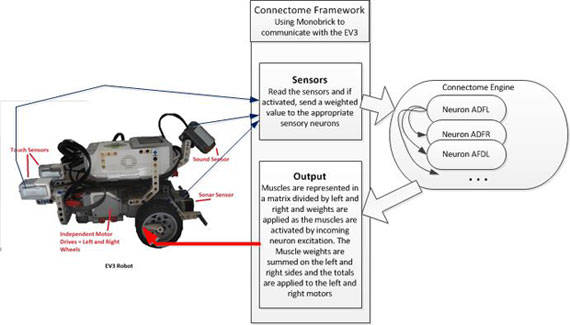
\includegraphics[width=\imsize]{connectomerobot.jpg}
	\caption[ Interacción Entre Sensores y Neuronas Motoras en el Robot de Timothy Busbice.]{  Interacción Entre Sensores y Neuronas Motoras en el Robot de Timothy Busbice. En esta figura se representa la interacción entre los sensores del robot construido por Timothy Busbice utilizando el Lego Mindstorms EV3 y el conectoma simulado del nematodo C. elegans. Un programa de entrada es responsable de activar las neuronas sensoriales correspondientes en el conectoma simulado en respuesta a las lecturas de los sensores del robot. Por otro lado, un programa de salida recopila las señales de las neuronas motoras y calcula valores ponderados que se utilizan para controlar las ruedas del robot, lo que resulta en su movimiento.  (Adaptada de \protect\cite{Timothy_robot} ).}\label{fig:timoty}
\end{figure}



Finalmente, inspirado en el trabajo de Timothy, Nathan Griffith ha concebido el proyecto \textquote{Nematoduino}, una simulación robótica del nematodo C. elegans compatible con Arduino Uno (El código esta disponible en \url{https://github.com/nategri/nematoduino}). Este proyecto se basa en un modelo de redes neuronales que utiliza un esquema de \textquote{leaky integrate-and-fire} del gusano biológico.  La implementación se caracteriza por una representación comprimida del conectoma (8 kilobytes) y la capacidad de ejecutarse en la plataforma económica y ampliamente disponible de Arduino Uno. A pesar de que el software \textquote{Nematoduino} consume una parte sustancial de la memoria y recursos del Arduino Uno, aún deja espacio para la personalización y experimentación. Con ruedas y un sensor de proximidad conectado a la placa, Nathan ha logrado imitar los movimientos y respuestas del gusano, como se puede apreciar en un video disponible en línea (\url{https://www.youtube.com/watch?v=u406m-v4Y3Y}).

Los esfuerzos en el campo de la neuro-robótica representan avances emocionantes al aplicar la biología computacional al diseño y control de sistemas robóticos, lo que podría tener un impacto significativo en el desarrollo de sistemas autónomos inspirados en la naturaleza, aspecto central en esta investigación doctoral.




\section{Discusión}



En este capítulo de la tesis, se presentan los fundamentos neurobiológicos del C. elegans, desde los experimentos realizados a nivel de toda la población neuronal, un modelo que integra la relación entre topología, función y comportamiento, hasta los modelos neurorrobóticos que podrían implementar físicamente estas características. Basándonos en el marco teórico anterior, en esta sección se presentan las preguntas que se desean resolver en los capítulos siguientes de esta parte de la tesis.

El nematodo Caenorhabditis elegans es un sistema modelo manejable para estudiar la locomoción, la navegación sensorial y la toma de decisiones. En su hábitat natural, se cree que navega por entornos multisensoriales complejos para encontrar comida y parejas sexuales, mientras evita amenazas como depredadores o entornos tóxicos. Si bien la investigación de las últimas décadas ha arrojado mucha luz sobre las funciones y los mecanismos de neuronas sensoriales seleccionadas, estamos al borde de comprender cómo la información sensorial es integrada por circuitos de interneuronas para la selección de acciones en el gusano. Los avances tecnológicos recientes han permitido la obtención de imágenes de \ce{Ca^{2+}} de todo el cerebro y de la actividad neuronal en gusanos que se mueven libremente.


Los animales que navegan por un entorno complejo no se limitan a reproducir los estímulos externos a través de sus acciones, sino que moldean su comportamiento en función de las condiciones. Los circuitos de quimiotaxis pueden transformar las entradas sensoriales suaves o ruidosas en reorientaciones discretas y probabilísticas. De manera más general, los animales toman decisiones y exploran entornos a través de acciones discretas y mutuamente excluyentes, que también son la base de paradigmas conductuales experimentales como las decisiones de ir/no ir o de elección forzada \cite{frederick_characterizing_2011}. Se hipotetiza que tanto las representaciones neuronales oscilatorias como las distribuidas son estrategias organizativas neuronales fundamentales, sobre las que quedan numerosas preguntas abiertas.

¿Cómo se relaciona el estado de actividad neuronal con el comportamiento? ¿Cómo se generan los patrones cíclicos y cómo coordinan su actividad las muchas neuronas de esta red? ¿Cuáles son las ventajas de estas implementaciones? ¿Cómo se integran la información sensorial, el aprendizaje y la historia del animal para cambiar la representación neuronal? Los experimentos presentados en los \Cref{sec:kato,sec:kaplan} respondieron a las anteriores preguntas al demostrar que la organización del comportamiento en el gusano está codificada en una estructura jerárquica de dinámica neuronal globalmente distribuida, continua y de baja dimensión, lo que lleva a la conclusión de que los estados de comportamiento están codificados en el cerebro como una representación interna que emerge del cerebro.

Para evaluar cómo se genera una actividad dinámica sostenida y de baja dimensión, es fundamental comprender el papel que juega el connectoma en la generación de movimiento rítmico. La estructura de la conectividad de una red neuronal a menudo determina cómo opera la red en su conjunto, codificando respuestas conductuales clave caracterizadas por patrones de actividad de baja dimensión. Sin embargo, la importancia exacta de la conectividad específica de una red no está clara, y la dinámica de la red neuronal a menudo se modela computacionalmente utilizando redes aleatorias uniformes. En C. elegans, sin embargo, la estructura del connectoma claramente no es aleatoria y puede desempeñar un papel crítico adicional en ayudar a generar o facilitar respuestas rítmicas. Esto se sugiere por el hecho de que los modelos computacionales del connectoma pueden generar oscilaciones de neuronas motoras relacionadas con la locomoción hacia adelante en respuesta a estímulos constantes, incluso sin propiocepción (e incluso cuando se modelan solo las dinámicas neuronales, sin modelado muscular, corporal o ambiental acoplado). Esto sugiere que las respuestas oscilatorias y estereotipadas están, en algún nivel, codificadas dentro del connectoma.


Por otro lado, la arquitectura de cableado de las redes neuronales se considera un determinante importante de sus cálculos dinámicos. Por lo tanto, un esfuerzo continuo en neurociencia es generar connectomas completos con resolución de sinapsis junto con mapas de actividad de todo el cerebro. Sin embargo, la relación estructura-función, es decir, cómo se relacionan el connectoma anatómico y la dinámica neuronal entre sí a escala global, sigue sin resolverse. Uzel et al. \cite{uzel_set_2022} compararon sistemáticamente las características de los grafos en el connectoma de C. elegans con las correlaciones en la dinámica neuronal de todo el sistema nervioso y encontraron que pocos motivos de conectividad local y principalmente otras características no locales, como los motivos de tripletes y las similitudes de entrada, pueden predecir relaciones funcionales entre neuronas. Sorprendentemente, cantidades como la fuerza de la conexión y la cantidad de entradas comunes no mejoran estas predicciones, lo que sugiere que la topología de la red es suficiente. Esto demuestra que las neuronas centrales en el connectoma son clave para estas características topológicas relevantes. De manera consistente, la inhibición de múltiples neuronas centrales interrumpe específicamente las correlaciones de todo el cerebro. Por lo tanto, los autores proponen que un conjunto de neuronas centrales y características de conectividad no locales proporcionan un sustrato anatómico para la dinámica cerebral global.


En los últimos años, el estudio de sistemas neuronales ha incorporado un nuevo paradigma que integra todo lo anteriormente expuesto, donde se considera la relación entre la información que procesa el cerebro, el cuerpo de los individuos y su interacción con el medio ambiente. Según este enfoque, el procesamiento de la información no puede considerarse de forma aislada en el cerebro, sino que debe hacerlo incorporando el estado dinámico del medio ambiente y cómo este es percibido por los diferentes sentidos propios de cada especie \cite{der_playful_2012}. Al mismo tiempo, otro de los grandes interrogantes en el estudio de las ciencias cognitivas y la inteligencia artificial está vinculado a la motivación que tienen los organismos para actuar de forma espontánea y cómo pueden diseñarse sistemas artificiales que actúen con una intención u objetivo sin que este tenga que estar programado de forma explícita \cite{brembs_towards_2010}.   Este paradigma resalta la importancia de estudiar el sistema nervioso, el cuerpo y el medio ambiente como un sistema acoplado, con el fin de comprender las propiedades que emergen de su interacción dinámica continua \cite{webb_robots_2002, floreano_robotics_2014}.  En este contexto, el uso de robots aparece como una herramienta de modelado atractiva, ya que es posible acceder y tener control total sobre los parámetros y variables dinámicas que gobiernan su comportamiento \cite{pfeifer_self-organization_2007}. Además, la implementación física de un robot permite probar el desempeño de algoritmos en un cuerpo sujeto a las leyes de la física e inmerso en tiempo real en un entorno natural, evitando así los complejos tecnicismos de la simulación del entorno, procedimiento que involucra sus propios modelos y, por lo tanto, agrega más variables, suposiciones y ruido al análisis. A su vez, esto nos permite centrarnos directamente en la dinámica global que emerge del connectoma y cómo afecta el comportamiento.


Tanto los resultados experimentales de Kato et al. \cite{kato_global_2015}, que muestran que la dinámica de la red interactúa con las neuronas sensoriales desde la primera sinapsis, proporcionando un andamiaje sólido para que las entradas sensoriales modulen el comportamiento, como los hallazgos del modelo del procesamiento sensoriomotor de Kaplan et al. \cite{kaplan_sensorimotor_2018}(\Cref{sec:modelo}) que muestran que la integración sensoriomotora en C. elegans ocurre de manera dinámica y distribuida, sugieren que la integración concurrente y distribuida de la dinámica sensorial y motora es un principio fundamental del funcionamiento del sistema nervioso. Por lo tanto, proponemos a C. elegans como un modelo manejable para estudiar las funciones y las ventajas computacionales de estas interacciones cerebro-cuerpo-entorno.

 Como se mencionó en el \Cref{sec:neurorobot}, Timothy Busbice, en línea con lo anterior, construyó un modelo de red neuronal utilizando como sustrato la información del connectoma del nematodo C. elegans. El robot presenta comportamientos emergentes que le permiten navegar espontáneamente cuando se estimulan las neuronas sensoriales asociadas con la presencia de alimentos y retroceder cuando se estimulan las neuronas de toque de la nariz al enfrentar un obstáculo. Es importante enfatizar que este comportamiento no fue programado intencionalmente en el robot, sino que surgió espontáneamente a partir del modelo de red neuronal y la interacción del robot con el medio ambiente.
 
 Pero ¿cómo emerge este comportamiento? Como objetivo general de esta parte de la tesis, buscaremos responder a este interrogante analizando las relaciones entre la estructura de red, la dinámica neuronal y el comportamiento emergente. Por tanto, el modelo robótico constituye una excelente plataforma para estudiar la interacción entre el connectoma, la dinámica neuronal y los comportamientos emergentes. Sin embargo, hasta ahora no se ha analizado ni la dinámica global del modelo ni su correlación con el connectoma subyacente y las acciones emergentes del robot.
 
 

 
 El primer objetivo específico busca cuantificar los comportamientos que emergen de un vehículo robótico que está controlado por una simulación numérica de red neuronal basada en el connectoma de C. elegans. En la simulación, las neuronas tienen el mismo umbral de activación y, en consecuencia, tienen una dinámica idéntica a la de las unidades aisladas. De esta manera, los cambios observados en su dinámica reflejan sus interacciones a través de la distribución no uniforme de la conectividad sináptica. Esto nos permite analizar la dinámica neuronal que emerge a través del connectoma y, al mismo tiempo, estudiar la interacción entre la dinámica neuronal y las acciones del robot. Esto proporciona una metodología para comprobar si las interacciones del circuito son suficientes para explicar el comportamiento o se necesitan más suposiciones. Primero reproduciremos los resultados publicados en C. elegans \cite{busbice_extending_nodate}. Luego analizaremos los comportamientos que emergen al manipular los circuitos más importantes del organismo real, asociados a la locomoción y la quimiosensación. La hipótesis de trabajo es que al implementar los circuitos funcionales en la red neuronal del robot, el robot tendrá comportamientos emergentes semejantes a los del organismo real.
 
 Al utilizar un modelo computacional para la dinámica del connectoma de C. elegans, proporcionamos un fuerte apoyo teórico y computacional para la hipótesis de que la propiocepción dentro de las neuronas motoras sí codifica e impulsa la actividad rítmica. El segundo objetivo busca caracterizar si algunos aspectos básicos de los comportamientos motores observados en el C. elegans están determinados por la estructura subyacente de la red neuronal asociada. Apoyados en estudios recientes que han demostrado que las redes biológicas, como el connectoma de C. elegans, tienen propiedades de redes complejas como mundo pequeño, caminos cortos entre dos nodos cualquiera, conexiones altamente agrupadas y principalmente motivos de red que podrían permitir procesamiento computacional canónico en números significativamente superiores a los de las redes aleatorias, proponemos la hipótesis de que esas características de red compleja, junto con una dinámica neuronal adecuada, permiten un comportamiento emergente, a diferencia de una red aleatoria que no tiene complejidad.
 
 El objetivo del experimento es comprobar que la estructura topológica de la red neuronal es necesaria para el comportamiento complejo del robot y no es un epifenómeno. Para corroborar esta hipótesis, se implementarán connectomas aleatorios en el robot para contrastar su resultado con el de la implementación con C. elegans.
 
 El tercer objetivo específico busca comprender cómo un sistema nervioso codifica, organiza y secuencia comportamientos. Se quiere ver si la dinámica neuronal global del gusano tiene la presencia de grupos de neuronas sincronizadas con una dinámica global de baja dimensión cíclica y estereotipada, como lo documentado en C. elegans reales. Para lograr esto, se realizarán experimentos monitorizando la dinámica neuronal global y aplicando las mismas técnicas que Kato et al. al conjunto de datos de la dinámica neuronal simulada. La hipótesis de trabajo es que en el robot se encontrará una actividad de red coordinada, al igual que en el organismo, como consecuencia de que la computación del comportamiento motor está implementada en el connectoma de C. elegans, tal como lo sugiere el modelo de Kaplan et al. (\Cref{sec.modelo})
 
 
 El cuarto objetivo específico busca comprender si la dinámica neuronal global del neurorobot también presenta una estructura jerárquica en los circuitos cerebrales y motores, donde las dinámicas más lentas limitan el estado y la función de las más rápidas, tal como en los experimentos en C. elegans. Nuestra hipótesis es que, a pesar de que todas las neuronas tienen el mismo umbral de activación y, por tanto, tienen una dinámica individual idéntica a la de las unidades aisladas, esperamos que su dinámica refleje la distribución no uniforme de la conectividad sináptica, dando como resultado una estructura jerárquica de frecuencias.
 
 En el siguiente capítulo se mostrarán los aspectos técnicos para la implementación de la dinámica neuronal de C. elegans en un robot. Se presentará el modelo de dinámica neuronal propuesto, los dos robots que implementarán esta dinámica y, finalmente, los métodos que se aplicarán sobre el resultado del comportamiento. El desarrollo de esta parte de la tesis tiene un alto impacto a nivel general, ya que intenta comprender la relación entre comportamientos emergentes en sistemas biológicos y la dinámica y estructura del cerebro, partiendo de un enfoque original que incorpora elementos de neurociencia experimental (connectomas), biología computacional (dinámica neuronal), sistemas complejos (comportamientos emergentes) y robótica (Arduino, Raspberry Pi). Este enfoque innovador abre la puerta a aspectos que nunca antes han sido considerados y se encontraron resultados novedosos, relevantes para el conocimiento científico en general y con alto impacto en todas estas áreas. Solo si podemos simular y manipular racionalmente un sistema nervioso, podremos comenzar a comprenderlo de verdad. Una vez más, el diminuto gusano de Brenner, que ocupa su lugar dulce único entre la simplicidad y la complejidad, se encuentra en la primera línea de los problemas más desafiantes de la biología.
 
 
\subsection{Hipótesis y Objetivos}
 
 \subsubsection{Hipótesis General}
 
 Se postula que la dinámica neuronal del nematodo C. elegans, basada en su connectoma, es un principio fundamental para el comportamiento emergente. Además, esta dinámica neuronal es replicable en un robot controlado por una red neuronal simulada, lo que permitirá comprender la relación entre el connectoma, la dinámica neuronal y los comportamientos emergentes.
 
 \subsubsection{Hipótesis Específica 1:}
 
 Se plantea que la implementación de circuitos funcionales del C. elegans en la red neuronal de un robot conducirá a comportamientos emergentes similares a los observados en el organismo real, respaldando la idea de que la propriocepción dentro de las neuronas motoras codifica e impulsa la actividad rítmica.
 
 \subsubsection{Hipótesis Específica 2:}
 
 Se sugiere que la estructura topológica de la red neuronal es un factor crítico para el comportamiento complejo del robot, en contraste con las redes aleatorias, lo que implica que las propiedades de redes complejas del connectoma de C. elegans son esenciales para el procesamiento computacional y el comportamiento emergente.
 
 \subsubsection{Hipótesis Específica 3:}
 
 La hipótesis sostiene que la dinámica neuronal global del robot mostrará una actividad de red coordinada, similar a la observada en C. elegans reales, debido a que la computación del comportamiento motor se basa en el connectoma del nematodo, según el modelo de Kaplan et al. \cite{kaplan_sensorimotor_2018}
 
 \subsubsection{Hipótesis Específica 4:}
 
 Se plantea que la dinámica neuronal global del neurorobot revelará una estructura jerárquica en los circuitos cerebrales y motores, donde las dinámicas más lentas limitan el estado y la función de las más rápidas, en concordancia con los experimentos en C. elegans.
 
 
 \subsection{Objetivos Generales y Específicos}
 
 Para abordar esta hipótesis general, se han formulado varios objetivos específicos:
 
 \subsection{Objetivo General}
 
 El propósito principal de esta investigación es comprender la relación entre el connectoma, la dinámica neuronal y los comportamientos emergentes, utilizando el nematodo C. elegans como modelo y replicando esta dinámica en un robot controlado por una red neuronal simulada.
 
 \subsubsection{Objetivo 1: Cuantificar Comportamientos Emergentes}
 
 El primer objetivo específico consiste en cuantificar los comportamientos emergentes en un vehículo robótico controlado por una simulación de red neuronal basada en el connectoma de C. elegans. Esto nos permitirá demostrar que la propriocepción dentro de las neuronas motoras codifica la actividad rítmica, respaldando así la hipótesis de trabajo.
 
 \subsubsection{Objetivo 2: Caracterizar la Estructura Topológica}
 
 El segundo objetivo específico se centra en caracterizar la importancia de la estructura topológica de la red neuronal en la generación de comportamientos complejos en el robot. Esto implica comparar la implementación de connectomas aleatorios con la del connectoma de C. elegans para corroborar la relevancia de las propiedades de redes complejas.
 
 
 \subsubsection{Objetivo 3: Analizar la Dinámica Neuronal Global}
 
 El tercer objetivo específico busca analizar la dinámica neuronal global del robot, examinando la presencia de grupos de neuronas sincronizadas con una dinámica de baja dimensión cíclica y estereotipada. Esto se hará en concordancia con los hallazgos en C. elegans y nos ayudará a comprender mejor la dinámica de la red neuronal.
 
 \subsubsection{Objetivo 4: Estudiar la Estructura Jerárquica de los Circuitos Cerebrales y Motores}
 
 El cuarto objetivo específico se enfoca en investigar si la dinámica neuronal global del neurorobot exhibe una estructura jerárquica en los circuitos cerebrales y motores. Esto incluye la evaluación de cómo las dinámicas más lentas limitan el estado y la función de las más rápidas, siguiendo los patrones observados en los experimentos con C. elegans.  
 
 Estos objetivos específicos se alinean con la hipótesis general y proporcionan un enfoque integral para la investigación. Cada objetivo contribuye a una comprensión más profunda de la dinámica neuronal y el comportamiento emergente en C. elegans y su replicación en un entorno robótico controlado por una red neuronal simulada. El estudio interconectado de estos objetivos nos permitirá avanzar hacia una comprensión más completa de la relación entre el connectoma, la dinámica neuronal y los comportamientos emergentes en estos sistemas biológicos y robóticos.
 
 
 



